% Copyright (C) 2014 by Thomas Auzinger <thomas.auzinger@cg.tuwien.ac.at>

\documentclass[draft,final]{vutinfth} % Remove option 'final' to obtain debug information.

% Extended LaTeX functionality is enables by including packages with \usepackage{...}.
\usepackage{fixltx2e}  % Provides fixes for several errors in LaTeX2e.
\usepackage{amsmath}   % Extended typesetting of mathematical expression.
\usepackage{amssymb}   % Provides a multitude of mathematical symbols.
\usepackage{mathtools} % Further extensions of mathematical typesetting.
\usepackage{microtype} % Small-scale typographic enhancements.
\usepackage{enumitem}  % User control over the layout of lists (itemize, enumerate, description).
\usepackage{multirow}  % Allows table elements to span several rows.
\usepackage{booktabs}  % Improves the typesettings of tables.
\usepackage[ruled,linesnumbered,algochapter]{algorithm2e} % Enables the writing of pseudo code.
\usepackage{nag}       % Issues warnings when best practices in writing LaTeX documents are violated.
\usepackage{hyperref}  % Enables cross linking in the electronic document version. This package has to be included second to last.
\usepackage[acronym,toc]{glossaries} % Enables the generation of glossaries and lists fo acronyms. This package has to be included last.
\usepackage{tikz}
\usetikzlibrary{decorations.pathmorphing}
\usepackage{listings}
\setsecnumdepth{subsection} % enumerate subsections

% Use an optional index
\makeindex
% Use an optional glossary
\makeglossaries
%\glstocfalse % remove the glossaries from the table of contents

% Set persons with 4 arguments:
%  {title before name}{name}{title after name}{gender}
%  where both titles are optional (i.e. can be given as empty brackets {})
\setauthor{}{Deniz Kocabas}{}{male}
\setadvisor{Priv.-Doz. Dr. }{Nysret MUSLIU}{}{male}

% For bachelor and master theses
% \setfirstassistant{Pretitle}{Forename Surname}{Posttitle}{male}
% \setsecondassistant{Pretitle}{Forename Surname}{Posttitle}{male}
% \setthirdassistant{Pretitle}{Forename Surname}{Posttitle}{male}

% For dissertations
\setfirstreviewer{Pretitle}{Forename Surname}{Posttitle}{male}
\setsecondreviewer{Pretitle}{Forename Surname}{Posttitle}{male}

% For dissertations at the PhD School
\setsecondadvisor{Pretitle}{Forename Surname}{Posttitle}{male}

% Required data
\setaddress{Embelgasse 5-7/6, 1050 Wien}
\setregnumber{1127055}
\setdate{23}{04}{2015}
\settitle{Exact Methods for Shift Design and Break Scheduling}{Exact Methods for Shift Design and Break Scheduling} % sets English and German version of the title (both can be English or German)
%\setsubtitle{Optional Subtitle of the Thesis}{Optionaler Untertitel der Arbeit} % sets English and German version of the subtitle (both can be English or German)

% Select the thesis type: bachelor / master / doctor / phd-school
% Bachelor:
% \setthesis{bachelor}
%
% Master:
\setthesis{master}
\setmasterdegree{dipl.} % dipl. / rer.nat. / rer.soc.oec. / master
%
% Doctor:
%\setthesis{doctor}
%\setdoctordegree{rer.soc.oec.}% rer.nat. / techn. / rer.soc.oec.
%
% Doctor at the PhD School
%\setthesis{phd-school} % Deactivate non-English title pages (see below)

% For bachelor and master
\setcurriculum{Software Engineering \& Internet Computing}{Software Engineering \& Internet Computing} % sets the English and German name of the curriculum

% For dissertations at the PhD School
\setfirstreviewerdata{Affiliation, Country}
\setsecondreviewerdata{Affiliation, Country}


\begin{document}

\frontmatter % switches to roman numbering
% The structure of the thesis has to conform to
%  http://www.informatik.tuwien.ac.at/dekanat

\addtitlepage{naustrian} % German title page (not for dissertations at the PhD School)
\addtitlepage{english} % English title page
\addstatementpage


\begin{abstract}
%% intro.tex
%% Copyright (C) 2014 by Thomas Auzinger <thomas.auzinger@cg.tuwien.ac.at>
%
% This work may be distributed and/or modified under the
% conditions of the LaTeX Project Public License, either version 1.3
% of this license or (at your option) any later version.
% The latest version of this license is in
%   http://www.latex-project.org/lppl.txt
% and version 1.3 or later is part of all distributions of LaTeX
% version 2005/12/01 or later.
%
% This work has the LPPL maintenance status `maintained'.
%
% The Current Maintainer of this work is Thomas Auzinger.
%
% This work consists of the files vutinfth.dtx and vutinfth.ins
% and the derived file vutinfth.cls.
% This work also consists of the file intro.tex.


\newacronym{ctan}{CTAN}{Comprehensive TeX Archive Network}
\newacronym{faq}{FAQ}{Frequently Asked Questions}
\newacronym{pdf}{PDF}{Portable Document Format}
\newacronym{svn}{SVN}{Subversion}
\newacronym{wysiwyg}{WYSIWYG}{What You See Is What You Get}

\newglossaryentry{texteditor}
{
  name={editor},
  description={A text editor is a type of program used for editing plain text files.}
}


Shift design and break scheduling problems that belong to class of NP-hard problems are variants of shift scheduling problem and are introduced recently in the literature. The shift scheduling problem today is very different from the one introduced by Dantzig \cite{li:1954:dantzig} and Edie \cite{li:1954:edie}. The relative importance of needed employees in scheduling decision has grown due to the economic considerations. Part time jobs, flexible work hours, lunch breaks and monitor breaks are the some of reasons to increase research attention.  

The shift design problem arises in a variety of large organizations. It involves efficient usage of personnel resources to reduce costs  as much as possible, while satisfying several constraints. Break scheduling problem is an important phase in the general employee scheduling in several organizations that needs a high level of concentration. The loss of concentration can end up with a dangerous consequences. It is important that the workers have from time to time breaks to keep the concentration level high. 

The purpose of the shift design problem is to find a minimum number of legal shifts, that reduce the shortages and excesses of workers in every time slots during the planning period. And in second part we assign the breaks within their shifts conveniently respect to several constraints and also keep the deviation of workforce for the timeslots as minimal as possible. We introduced integer linear programming formulation explicitly for solving shift design and break scheduling problems. The explicit model is investigated based on enumeration of each shift or break from the possible shift or breaks starts and  lengths. For break scheduling, due to the large number of constraints and variables, we restricted the problem definition. 

The simplex algorithm and branch and bound search are performed by the Cplex and Gurobi Solver, to solve the integer programming model for the data sets of shift design problem. The Cplex Solver shows faster performance compared to Gurobi Solver. Therefore, we continue our experiments using only Cplex Solver. We tried different parameters in Cplex Solver, with the instances exceed 2 hours time limit for the shift design problem. These parameters speed up the process, meanwhile change the optimality tolerance. 

Exact method shows also superior performance for break scheduling problem with using Cplex Solver. However, our formulation fails to run in the real life instances of break scheduling problem, due to our restrictions in this problem. We improved the previous solutions and obtained the best known results in the state-of-the-art for both shift design and break scheduling problem. 

 
\end{abstract}

\begin{acknowledgements*}
%% intro.tex
%% Copyright (C) 2014 by Thomas Auzinger <thomas.auzinger@cg.tuwien.ac.at>
%
% This work may be distributed and/or modified under the
% conditions of the LaTeX Project Public License, either version 1.3
% of this license or (at your option) any later version.
% The latest version of this license is in
%   http://www.latex-project.org/lppl.txt
% and version 1.3 or later is part of all distributions of LaTeX
% version 2005/12/01 or later.
%
% This work has the LPPL maintenance status `maintained'.
%
% The Current Maintainer of this work is Thomas Auzinger.
%
% This work consists of the files vutinfth.dtx and vutinfth.ins
% and the derived file vutinfth.cls.
% This work also consists of the file intro.tex.


\newacronym{ctan}{CTAN}{Comprehensive TeX Archive Network}
\newacronym{faq}{FAQ}{Frequently Asked Questions}
\newacronym{pdf}{PDF}{Portable Document Format}
\newacronym{svn}{SVN}{Subversion}
\newacronym{wysiwyg}{WYSIWYG}{What You See Is What You Get}

\newglossaryentry{texteditor}
{
  name={editor},
  description={A text editor is a type of program used for editing plain text files.}
}

Foremost, I would like to express my sincere gratitude to my supervisor Priv.-Doz. Dr. Nysret Musliu for the continuous support of my master thesis, for his patience, motivation, enthusiasm, and immense knowledge. His guidance and constructive critism helped me in all the time of research and writing of this thesis. I could not have imagined having a better advisor and mentor for my master thesis. \\

Besides my advisor, I would also like to thank the rest of the people of the Department for their help and support. \\

Last but not the least, I would like to thank my family, especially to my father Mehmet Kocabas and my mother Ummuhan Kocabas, for supporting me throughout my life. 
\end{acknowledgements*}



% Select the language of the thesis, e.g., english or naustrian.
\selectlanguage{english}

% Add a table of contents (toc)
\tableofcontents % starred version, i.e., \tableofcontents*, removes the self-entry

% Use an optional list of figures
\listoffigures % starred version, i.e., \listoffigures*, removes the toc entry

% Use an optional list of tables
\listoftables % starred version, i.e., \listoftables*, removes the toc entry

% Use an optional list of alogrithms
\listofalgorithms
\addcontentsline{toc}{chapter}{List of Algorithms}

% Switch to arabic numbering and start the enumeration of chapters in the table of content.
\mainmatter

\chapter{Introduction}
%% intro.tex
%% Copyright (C) 2014 by Thomas Auzinger <thomas.auzinger@cg.tuwien.ac.at>
%
% This work may be distributed and/or modified under the
% conditions of the LaTeX Project Public License, either version 1.3
% of this license or (at your option) any later version.
% The latest version of this license is in
%   http://www.latex-project.org/lppl.txt
% and version 1.3 or later is part of all distributions of LaTeX
% version 2005/12/01 or later.
%
% This work has the LPPL maintenance status `maintained'.
%
% The Current Maintainer of this work is Thomas Auzinger.
%
% This work consists of the files vutinfth.dtx and vutinfth.ins
% and the derived file vutinfth.cls.
% This work also consists of the file intro.tex.


\newacronym{ctan}{CTAN}{Comprehensive TeX Archive Network}
\newacronym{faq}{FAQ}{Frequently Asked Questions}
\newacronym{pdf}{PDF}{Portable Document Format}
\newacronym{svn}{SVN}{Subversion}
\newacronym{wysiwyg}{WYSIWYG}{What You See Is What You Get}

\newglossaryentry{texteditor}
{
  name={editor},
  description={A text editor is a type of program used for editing plain text files.}
}


\section{Motivation}

In this thesis, we investigated an integer programming approach to solve two NP-hard problems, shift design and break scheduling. These two problems are variants of the shift scheduling problem and are introduced recently in the literature. The shift scheduling problem has been first introduced by Edie (1954 )\cite{li:1954:edie} in the context of toll booth operators scheduling. Solving this shift scheduling problem was originally proposed by Dantzig \cite{li:1954:dantzig} by the set covering formulation. The shift scheduling problem today is very different from the one introduced by Dantzig \cite{li:1954:dantzig} and Edie \cite{li:1954:edie}. The relative importance of needed employees in scheduling decision has grown due to the economic considerations. Part time jobs, flexible work hours, lunch breaks and monitor breaks are the some of reasons to increase research attention. The motivations of the shift design and the break scheduling problems are presented below separately in two sections.

\subsection{Shift Design}

The shift design problem arises in a variety of large organizations such as airlines, hospitals, telephone companies, police departments, etc. It involves efficient usage of personnel resources to reduce costs  as much as possible, while meeting several constraints. The professional planners can construct solution for small practical problems by hand, but for the large number of different demands and solutions, the solution space is too large for an efficient manual approach. Even though finding a solution manually is possible, it is unlikely, that the optimum solution will be found. Furthermore, finding a solution manually usually takes very long time \cite{li:2013:gaspero}. Therefore, different approaches in the literature \cite{li:2004:musliu} \cite{li:2007:gaspero} \cite{li:2013:gaspero} \cite{li:2010:abseher} have been proposed to solve this problem.

\subsection{Break Scheduling}

The break scheduling problem is an important phase in the general employee scheduling in several organizations that needs a high level of concentration, such as air traffic control, security checking, supervision, assembly line workers, etc. The loss of concentration in such organization can end up with a dangerous consequences. It is necessary that the workers have from time to time breaks to keep the concentration level high. 

In the break scheduling problem, breaks need to be assigned to shifts over one week. The slot length is usually 5 minutes, therefore, huge number of possible assignments of breaks exist. Due to the problem's size and complexity, to calculate optimum breaks for large number of shifts is impossible. Automatic or computer aided break scheduling is usually the only way to reach high quality shift plans. Therefore, this problem has been considered by researchers in the literature \cite{li:2008:beer} \cite{li:2010:beer} \cite{li:2014:widl}.

The aim of this master thesis is to investigate new solution techniques for shift design and break scheduling problems. We will introduce an integer programming approach for solving shift design and break scheduling. The integer programming formulation for shift design and break scheduling problem is expected to find optimal solutions for many instances or at least to improve the existing results.


\section{Aim of The Work}

The aim of our thesis consists of four main parts:

\begin{itemize}

\item The integer programming formulation will be proposed for shift design and break scheduling problems. We plan to study different formulations for both problems.

\item To solve the models, we will apply the Cplex Solver and Gurobi Solver. We will compare experimentally the two solvers on benchmark instances for shift design problem from the literature.

\item For experimentations, different parameters in Cplex Solver will be used. These parameters speed up the process, meanwhile change the optimality tolerance.

\item To measure the performance of an integer programming approach, the results will be compared with the existing state-of-the-art's results in the literature. 
\end{itemize}

\section{Results of the Master's Thesis}

We obtained the results of this master thesis are given as follows,

\begin{itemize}

\item We propose an integer linear formulation for shift design and break scheduling problems. For break scheduling, due to the large number of constraints and variables, we restricted the problem definition.

\item Cplex Solver obtains the results in less time compared to Gurobi Solver for datasets of the shift design problem.

\item In a few instances of shift design problem, we could not obtain results in 2 hours time limit and for these instances three different parameters of Cplex Solver are performed. By using these parameters, we can not guarantee the optimal solution is found. However, these long lasting instances by using these parameters also achieved better solutions compared to previous results. 

\item We compare our algorithms with the best existing results for the both problems in literature. We obtained the best existing result in each instance (except one). However, our formulation fails to run in the real life instances of break scheduling problem, due to our restrictions in this problem.
\end{itemize}


\section{Structure of the Master's Thesis}

The remaining parts of this thesis are organized into the following chapters: 

\begin{itemize}
\item In \textbf{Chapter 2}, we will introduce the shift design and the break scheduling problem. The formal definition of shift design and break scheduling problems, that we have solved in this thesis, are given. 

\item In \textbf{Chapter 3}, we will give an overview of state-of-the-art. We will discuss the proposed integer linear programming formulations for a similar problem called shift scheduling problem and then we will give the related work for shift design and break scheduling problems. 

\item In \textbf{Chapter 4}, we will present our integer linear programming formulations for both problems in details. The variables, constraints and objective functions will be described. 

\item In \textbf{Chapter 5}, we will present the computational results obtained by our integer linear programming formulations for shift design and break scheduling problems. We will compare the two integer linear programming solvers, Cplex Solver and Gurobi Solver for the datasets of shift design problem. We will experiment different parameters in Cplex Solver for long lasting instances of shift design problem. At last, we will compare our results with the best known result in the state-of-the-art for both problems.

\item In \textbf{Chapter 6}, we conclude this thesis by summarizing the work presented and give ideas for potential future work.

\end{itemize} 

\chapter{Problem Statements}
%% intro.tex
%% Copyright (C) 2014 by Thomas Auzinger <thomas.auzinger@cg.tuwien.ac.at>
%
% This work may be distributed and/or modified under the
% conditions of the LaTeX Project Public License, either version 1.3
% of this license or (at your option) any later version.
% The latest version of this license is in
%   http://www.latex-project.org/lppl.txt
% and version 1.3 or later is part of all distributions of LaTeX
% version 2005/12/01 or later.
%
% This work has the LPPL maintenance status `maintained'.
%
% The Current Maintainer of this work is Thomas Auzinger.
%
% This work consists of the files vutinfth.dtx and vutinfth.ins
% and the derived file vutinfth.cls.
% This work also consists of the file intro.tex.


\newacronym{ctan}{CTAN}{Comprehensive TeX Archive Network}
\newacronym{faq}{FAQ}{Frequently Asked Questions}
\newacronym{pdf}{PDF}{Portable Document Format}
\newacronym{svn}{SVN}{Subversion}
\newacronym{wysiwyg}{WYSIWYG}{What You See Is What You Get}

\newglossaryentry{texteditor}
{
  name={editor},
  description={A text editor is a type of program used for editing plain text files.}
}

In this chapter, the formal definition of shift design and break scheduling problems, that we have solved in this thesis, are given. 


\section{Shift Design Problem}
Below we give the definition of the shift design problem. Our description is based on the problem definition from \cite{li:2001:gärtner} \cite{li:2004:musliu}:

\begin{itemize}
\item Planning period consists of $n$ consecutive time slot $[a_1,a_2), [a_2,a_3), . . . , [a_n,a_{n+1})$, all having the same length $slotlength$ in minutes. The needed number of workers $w_i$ for each interval $[a_i, a_{i+1})$. The shift design problem has a cyclic structure, therefore the end of the planning period $a_{n+1}$ is equal to the first time point $a_1$. The format of time points is: $day:hour:minute$

\item The shifts can be generated depending on $y$ shift types $v_1,...,v_y$. Each shift type has a minimum/maximum start and  minimum/maximum length. 
\begin{itemize}
\item[] $v_j.minStart :$  Earliest start of the shift types $j$. 
\item[] $v_j.maxStart :$ Latest start of the shift types $j$. 
\item[] $v_j.minLength :$  Shortest duration of the shift types $j$. 
\item[] $v_j.maxLength :$  Longest duration of the shift types $j$. 
\end{itemize}

In Table~\ref{tab:shifttypes} an example of four shift types is given.

\item In original definition of shift design problem, there are also two scalar real-valued quantities, used to define the distance from the average number of duties. 

\begin{itemize}
\item[] AS : The upper limit for the average number of working shifts per week per employee.
\item[] AH : Average number of working hours per week per employee.
\end{itemize}

These two parameters are not used in our integer programming formulation.

\end{itemize}

\begin{table}
  \centering
  \begin{tabular}{ccccc}
    \toprule
    Shift type & MinStart         & MaxStart      & MinLength & MaxLength        \\
    \midrule
    M     & 05:00	 & 08:00          & 07:00 	& 09:00        \\
    D     & 09:00	 & 11:00          & 07:00	& 09:00        \\
    A     & 14:00	 & 16:00          & 07:00	& 09:00        \\
    N     & 21:00	 & 23:00          & 07:00	& 09:00        \\
    \bottomrule
  \end{tabular}
  \caption{An example of shift types}
  \label{tab:shifttypes} 
\end{table}

The purpose of the shift design problem is to generate $k$ shifts $s_1, s_2,...s_k$, which belongs to one of the shift types. Every shift has a start point $v_j.start$ and length $v_j.length$ parameters.  Additionally, each real shift $s_p$ has adjoined parameters $s_p.w_i, \forall i \in \{1,...,C\}$ (C represents the number of days in the planning period and usually considered a week) representing the number of workers in shift $s_p$ during the day $i$. The aim is to minimize the four components given below:

$F_1$ : Sum of the excesses of workers in each time slot during the planning period

$F_2$ : Sum of the shortages of workers in each time slot during the planning period

$F_3$ : Number of shifts

$F_4$ : Distance of the average number of duties per week in case it is above a certain threshold. This component is meant to avoid an excessive fragmentation of workers load in too many short shifts.

This is a multi criteria optimization problem. Unlike the four weighted components in the original definition, we have used the first three like in the article \cite{li:2007:gaspero}. These remaining three components have different importance depending on the situation. 

As we mentioned above, we avoided some of the instances, that are necessary to calculate the distance of the average number of duties per week per employee. To disregard this fourth component of the objective function is reducing the complexity of the problem statement. This criterion is also excluded in \cite{li:2007:gaspero}.

The formal representation of the shift design problem is given in detail in the article \cite{li:2001:gärtner} \cite{li:2004:musliu}.

\section{Break Scheduling Problem}

Below we give the definition of break scheduling problem. Our description is based on the problem definition from \cite{li:2010:beer}:

\begin{itemize}

\item Planning period divided into $n$ consecutive time slot $[a_1,a_2), [a_2,a_3), . . . , [a_n,a_{n+1})$, all with the same length $slotlength$ usually 5 minutes. The break scheduling problem has also cyclic structure, therefore the last time slot $t_{n+1}$ is equal to the first time slot $t_1$.

\item There are $k$ shifts $(s_1, s_2, ..., s_k)$, indicating the work schedule of employees. The break time per shift $s_i$ is calculated based on the shift length. If shift length is less or equal to 10 hours, break time is,

\begin{equation}
s_i.breakTime = floor( ( minutes(Shift Length) - 20) / 50 ) * 10
\end{equation}

otherwise,
\begin{equation}
s_i.breakTime = ceil (   minutes(Shift Length) / 4 )
\end{equation}

\item The employee requirements for each time slot, $[a_1,a_2), [a_2,a_3), . . . , [a_n,a_{n+1})$ in the planning period are defined as follows,

\begin{itemize}
\item $w_t$ is the needed number of workers  for the time slot $t$.
\item A staff is considered to be working for the time slot $t$, if the time slot $t$ is in the employees working schedule and the employees are not in the break period in time slot $t$.
\item An employee needs a full time slot (typically 5 minutes) to return back to work after a break. Thus, the first time slot after the break, the staff is not considered to be working.
\end{itemize}

\item Shifts and breaks have two parameters, that are the beginning or ending time points of shifts or breaks. The duration value can be calculated by substracting the time slots of the $start$ and $end$ of shifts or breaks. Moreover, each break is associated with a certain shift in which it is scheduled. We distinguish between two different types of breaks, that are monitor or lunch breaks.

\end{itemize}

Given a planning period, a set of shifts, the associated total break times, and the staffing requirements, there are several hard and soft constraints, that need to be considered for the break scheduling problem. The hard constraints are:
\begin{itemize}
\item Each break lies entirely within its associated shift.

\begin{equation}
s_i.start \le b_j.start \le b_j.end \le s_i.end
\end{equation}

\item Two distinct breaks associated with the same shift, do not overlap in time. 

\begin{equation}
 b_j.start \le b_j.end \le  b_k.start \le b_k.end 
\end{equation}

or

\begin{equation}
 b_k.start \le b_k.end \le  b_j.start \le b_j.end 
\end{equation}

\item Sum of break durations needs to be equal to shift's break time. 

\begin{equation}
\sum_{b_j \in s_i} b_j.duration = s_i.breakTime
\end{equation}


\end{itemize}

Among, all feasible solutions for the break scheduling problem, there are seven soft constraints. These constraints are useful to assign the breaks within their shifts conveniently and to reduce the excesses and shortages of workforce for the time slots. These seven criteria are explained below, \\

$C_1$: Break Positions. Each break, $b_j$, may start, at the earliest, a certain number of time slots after the beginning of its associated shift $s_i$, and may end, at the latest, a given number of time slots before the end of its shift:

\begin{equation}
b_j.start \ge s_i.start + distanceToShiftStart
\end{equation}

\begin{equation}
b_j.end \le s_i.end + distanceToShiftEnd
\end{equation}


$C_2$: Lunch Breaks. A shift $s_i$ can have several lunch breaks, each required to last a specified number of time slots (min lunch break duration), and should be located within a certain time window after the shift start. Let $b_{lb}$ be a lunch break. Then,

\begin{equation}
b_{lb}.start \ge s_i.start + distanceToShiftStartLB
\end{equation}

\begin{equation}
b_{lb}.end \le s_i.end + distanceToShiftEndLB
\end{equation}

$C_3$: Duration of Work Periods. Breaks divide a shift into several work and rest periods. The duration of work periods within a shift must range between a required minimum and maximum duration:

\begin{equation}
minWorkDuration \le b_1.start - s_i.start \le maxWorkDuration
\end{equation}

\begin{equation}
minWorkDuration \le b_{j+1}.start - b_j.end \le maxWorkDuration
\end{equation}

\begin{equation}
minWorkDuration \le s_i.end - b_m.end  \le maxWorkDuration
\end{equation}

where $(b_1,...,b_j,b_{j+1},...,b_m)$ are the breaks of $s_i$ in temporal order.

$C_4$: Minimum Break Times after Work Periods. If the duration of a work period exceeds a certain limit, the break following that period must last a given minimum number of time slots ($minTsCount$):

\begin{equation}
 b_1.start - s_i.start \ge workLimit  \Rightarrow b_1.duration \ge minTsCount
\end{equation}

\begin{equation}
 b_{j+1}.start - b_j.end \ge workLimit  \Rightarrow b_{j+1}.duration \ge minTsCount
\end{equation}



$C_5$: Break Durations. The duration of each break, $b_j$, must lie within a specified minimum and maximum value:

\begin{equation}
minDuration \le b_j.duration \le maxDuration
\end{equation}

$C_6$: Shortage of Employees. At least $w_t$ employees should be working in each time intervals, $[a_t, a_{t+1})$. Sum of the shortages of workers in each time slot during the planning period indicating the $C6$.

$C_7$: Excess of Employees. At most $w_t$ employees should be working in each time intervals $[a_t, a_{t+1})$.  Sum of the excesses of workers in each time slot during the planning period indicating the $C7$.


This is also a multi criteria optimization problem. For each soft constraint, we have weight value. These weights can be different depending on the situations. Given an instance of the break scheduling, our goal is to find a feasible solution, with minimizing the soft constraints. 

\chapter{Related Work}
%% intro.tex
%% Copyright (C) 2014 by Thomas Auzinger <thomas.auzinger@cg.tuwien.ac.at>
%
% This work may be distributed and/or modified under the
% conditions of the LaTeX Project Public License, either version 1.3
% of this license or (at your option) any later version.
% The latest version of this license is in
%   http://www.latex-project.org/lppl.txt
% and version 1.3 or later is part of all distributions of LaTeX
% version 2005/12/01 or later.
%
% This work has the LPPL maintenance status `maintained'.
%
% The Current Maintainer of this work is Thomas Auzinger.
%
% This work consists of the files vutinfth.dtx and vutinfth.ins
% and the derived file vutinfth.cls.
% This work also consists of the file intro.tex.


\newacronym{ctan}{CTAN}{Comprehensive TeX Archive Network}
\newacronym{faq}{FAQ}{Frequently Asked Questions}
\newacronym{pdf}{PDF}{Portable Document Format}
\newacronym{svn}{SVN}{Subversion}
\newacronym{wysiwyg}{WYSIWYG}{What You See Is What You Get}

\newglossaryentry{texteditor}
{
  name={editor},
  description={A text editor is a type of program used for editing plain text files.}
}


In this section, we will give an overview of state of the art in the area of shift design and break scheduling. The variants of problems, we solved in this thesis are introduced recently in the literature. However a similar problem called shift scheduling problem usually with a break or multiple breaks has been extensively investigated in the literature. We will first give the related work for the shift scheduling problem and then we will give the state of the art for shift design and break scheduling problems.

\section{Shift Scheduling with Breaks}

Different approaches have been proposed for the shift scheduling problem, especially based on integer programming formulation. The problem has been first introduced by Edie (1954) \cite{li:1954:edie} in the context of toll booth operator scheduling. Solving this shift scheduling problem was originally proposed by Dantzig  \cite{li:1954:dantzig} by the set covering formulation. 

The integer programming model of Dantzig is given below:

\begin{equation}
\min \sum_{j=1}^n c_j * x_j
\end{equation}
subject to:

\begin{equation}
\sum_{j=1}^n a_{tj} x_j \ge b_t \quad \forall t = 1, 2, ...m
\end{equation}
\begin{equation}
x_{j} \ge 0, \quad x \in \mathbb{Z} \quad \forall j = 1, 2, ...n 
\end{equation}
\\ where,

$n$ : number of possible shifts.

$m$ : number of time slot in the planning period.

$c_{j}$ : cost of assigning an employee to shift $j$.

$x_{j}$ : number of workers assigned to shift $j$.

$a_{tj}$ : is 1, if time slot $t$ is a work period for shift $j$, 0 otherwise.

$b_t$ : needed number of employees in time slot $t$. \\

The solution of this formulation can be found by enumerating the feasible shifts based on possible shift starts, shift durations, breaks, and time windows for breaks. However, involving a high flexibility with including different shift start times, lengths, multiple breaks, multiple break types cause increasing the number of enumerated shifts. For this reason, to solve with the explicit set covering formulation can be very difficult.

Researchers have proposed different formulations to overcome this difficulty. Moondra \cite{li:1976:moondra} proposed an approach of implicitly representing shifts. The considered model has two types of shifts; full-time and part-time:

\begin{itemize}
\item Full-time shifts: Fixed length and a lunch break window allowing two break starting times. To assign the break placements, half of the employees take their lunch in the first period and the remaining half of workers in the second break period.
\item Part-time shifts: with a length variable (4-8 hours) and no lunch break. The  length of the part-time shift was represented implicitly. 
\end{itemize}

Bechtold and Jacobs \cite{li:1990:bechtold} introduced a new integer formulation, that break assignments were modeled implicitly rather than explicitly. The formulation considers a single break with the same duration in each shift. Although the extended formulation was shown to be superior compared to the set covering model, approach is restricted to the less than 24 hours planning period. Thompson \cite{li:1995:thompson} combined these two formulation works of Moondra \cite{li:1976:moondra} and Bechtold and Jacobs \cite{li:1990:bechtold} to achieve a fully implicit formulation of the shift scheduling problem. This formulation reduces the size and improve the scheduling flexibility.

Aykin \cite{li:1996:aykin} proposed an implicit integer programming model with LINDO for the shift scheduling problem with break placement. The problem is extended that employees have multiple rest breaks and a lunch break. The length of a lunch break is usually 30 to 60 minutes and a rest break is 15 to 30 minutes. The proposed formulation has also time window for lunch and rest breaks. For instance, Aykin assumed that time window of a break starts half an hour before the ideal break location and take 90 minutes. Therefore, 6 possible different time slots to assign 15 minute break and 5 different ways for a 30 minute break. It reduces the number of variables needed. The approach is not only feasible for less than 24 hours planning period, but also suitable for 24 hours continuous (cyclical problem) planning period. 

Aykin \cite{li:2000:aykin} extended Bechtold and Jacobs's formulation \cite{li:1990:bechtold} a generalized version by relaxing the assumptions of it and compared with the model that he presented in  \cite{li:1996:aykin}. Although generalized version of Bechtold and Jacobs's approach has fewer variables, it has more constaints and more non- zero in A-matrix. Its end up with a worse performance than the model of Aykin.

To overcome the difficulties by explicit set covering formulation, implicit models have been used to solve shift scheduling problems efficiently. However, implicit models use more complex formulations to assign feasible shifts. These approaches have some problems in solving large size problems. This difficulties lead researchers to propose approaches either using branch and price \cite{li:2000:mehrotra}  or using branch and cut approach \cite{li:1998:aykin}. Aykin \cite{li:1998:aykin} proposed branch and cut algorithm based on an implicit formulation for the shift design problem. Rounding heuristic is used to add cuts and updated iteratively. Mehrotra et al. \cite{li:2000:mehrotra} developed a branch and price approach. Their formulations obtained good results for the large shift scheduling problems, optimal solutions or best non-optimal solutions were found.  

Rekik et al. \cite{li:2010:rekik} proposed an implicit formulation of the shift scheduling with multiple breaks. To increase flexibility, fractionable breaks and work stretch duration restriction are used. Each break is appropriately assigned by minimum and maximum pre- and post-break work stretch duration constraints. Breaks can  be divided into fractional breaks and this sub breaks can have different lengths, depends on minimum, maximum sub break lengths and the sum of the lengths of sub break is equal to the total break duration of the shift.


\section{Shift Design}

The concept of shift design has been first introduced in \cite{li:2001:gärtner} \cite{li:2004:musliu} \cite{li:2001:musliu}. There are several differences, that characterize the shift design problem. The shifts are generated over multiple days, usually a week, rather than a day. The shift design problem has a cyclic structure, therefore the last time slot of the week is connected to the first time slot of a week. In order to minimize the number of shifts in shift design problem, we need to consider reusing shifts on all days of the week. Furthermore, the objective function of shift scheduling is to minimize the number of workers, without any shortages of employees. 

In these first publications; Musliu et al. proposed a local search approach with a set of move types to explore the neighbourhood. In order to avoid cycles in the move selection process, tabu search mechanism is used. To make the search more effective, the neighbourhood exploration mechanism is based on analyzing the distance of the current solution to the optimal solution with respect to the shortages or excesses of workers with the longest duration and the used shift types. The initial solution of the algorithm is based on to consider every change of the requirements. These differences of consecutive time slot can be beginning (increase of requirement) or ending (decrease of requirement) point of a shift. 

Di Gaspero et al. \cite{li:2007:gaspero} improved this method and composed a greedy construction heuristic with the local search algorithm. The initial solution is constructed using new greedy heuristic based on min-cost max-flow. Shifts are edges and workforces are the edge flows. In the second stage, the local search paradigm is used to explore the neighbourhood. The hybrid solver outperforms the previous approach. Abseher \cite{li:2010:abseher} proposed different modelling approaches using answer set programming, but the performance could not be improved obtained by solving the shift design problem using the heuristic-based approaches in \cite{li:2007:gaspero}.

\section{Break Scheduling}

Beer et al. \cite{li:2008:beer} introduced the break scheduling problem, that presented in the previous chapter and developed local search techniques based on min-conflicts algorithm. Although min-conflict search tries to improve the solution incrementally by concentrating on violating constraints, is not being able to escape from local optima. Random walk strategy is adapted to explore further regions with a probability p and the remaining 1-p probability is used for min-conflict search. Tabu search mechanism and simulated annealing algorithm \cite{li:2010:beer} are implemented and the performances compared with min-conflicts-random-walk search. The min-conflicts-random-walk approach outperformed the other two heuristic techniques.

Widl  \cite{li:2009:widl} introduced a memetic algorithm for break scheduling problem. Initial solutions were constructed randomly or by fast heuristic. Break patterns created and remained unviolated the constraints $C_1$ -$ C_5$   during each iteration. Every individual tries to find the best solutions with using a local search algorithm. This approach improved the previous results based on min-conflicts-random-walk for the break scheduling problem. 

Widl  \cite{li:2014:widl} \cite{li:2010:widl} \cite{li:2010:widlimp} proposed 2 new memetic algorithms. These approaches are used a new memetic representation based on time periods instead of on each shift, therefore these algorithms require different genetic operators. In the first algorithm, tabu search is used to prevent re-visiting old computed solutions in local search. To improve the first algorithm, crossover operator is developed in the second algorithm, that every offspring can have more than one parent and each individual can be parent also. With each iteration, the first offspring is created by joining the best memes of the current memepool and the remaining are created by applying a k-tournament. Bad individuals are less likely to be discarded. To calculate the best memes and to discard some individuals, penalty system was developed. As a result, applying local search for some instances instead of all of them provided a better result. The approach obtain the best results for the break scheduling problem.

\section{Shift Design and Break Scheduling}

Real life shift design and break scheduling problem arise in different areas of industry. Generally in the literature, the break scheduling has been addressed mainly as part of the shift scheduling problem. Such an example, which have multiple rest breaks and a lunch break, we presented before, is proposed by Aykin \cite{li:1996:aykin}. 

G\"artner et al. \cite{li:2005:gaertner} extended shift design problem first time with breaks. The break scheduling definition is described differently as we presented in Chapter 2 before. There are fewer soft constraints, which are minimal and maximal length of break, minimal and maximal distance of start of break from the shift begin, and minimal distance of end of break from the end of the shift. One or more breaks can be assigned to every shifts. The shifts are generated first based on local search, that we presented above (\cite{li:2001:gärtner} \cite{li:2004:musliu}). The solution found by local search converted to shifts with one employee per day and greedy algorithm was used to assign breaks. The greedy algorithm finds the best position of the breaks depend on under- and over-covers. Next step is to update the length of breaks or shifts to increase or decrease to improve solution. Last step creates the solution with shifts and multiple employees. The algorithm found an average solution. 

G\"artner et al. \cite{li:2006:gaertner} improved this algorithm by using integer programming formulation based on the set covering model of Dantzig  \cite{li:1954:dantzig} for shift design phase, rather than local search. The shift design problem was defined with an extra component compared to the shift design problem presented in this master thesis, that is the sum of the deviations of the shift lengths from the optimal shift length. Same steps were used for assigning breaks with the previous article \cite{li:2005:gaertner}. The method gave good results in practice. 

Di Gaspero et al. \cite{li:2010:gaspero} \cite{li:2013:gaspero} proposed an innovative hybrid method that combines features of local search and constraint programming  techniques. The problem is divided into two sub problems, where the local search technique is used to determine the shifts in the first phase and the constraint programming model to assign breaks. This approach could not improve the results obtained by solving the break scheduling problem separately after generating shifts. 
 

\chapter{Formulations}
%% intro.tex
%% Copyright (C) 2014 by Thomas Auzinger <thomas.auzinger@cg.tuwien.ac.at>
%
% This work may be distributed and/or modified under the
% conditions of the LaTeX Project Public License, either version 1.3
% of this license or (at your option) any later version.
% The latest version of this license is in
%   http://www.latex-project.org/lppl.txt
% and version 1.3 or later is part of all distributions of LaTeX
% version 2005/12/01 or later.
%
% This work has the LPPL maintenance status `maintained'.
%
% The Current Maintainer of this work is Thomas Auzinger.
%
% This work consists of the files vutinfth.dtx and vutinfth.ins
% and the derived file vutinfth.cls.
% This work also consists of the file intro.tex.


\newacronym{ctan}{CTAN}{Comprehensive TeX Archive Network}
\newacronym{faq}{FAQ}{Frequently Asked Questions}
\newacronym{pdf}{PDF}{Portable Document Format}
\newacronym{svn}{SVN}{Subversion}
\newacronym{wysiwyg}{WYSIWYG}{What You See Is What You Get}

\newglossaryentry{texteditor}
{
  name={editor},
  description={A text editor is a type of program used for editing plain text files.}
}

In this chapter, we will present our integer programming formulation for shift design and break scheduling problems in details.  The integer programming approach is explained separately in two subsections. In each subsection, we describe the variables that we used, the constraints and the objective function. 

\section{Integer Linear Programming Model for Shift Design Problem}

The explicit set covering formulation have been first proposed for the shift scheduling problem by Dantzig (1954) \cite{li:1954:dantzig}. Our integer programming formulation is also based on an explicit representation of shift design. To formulate the shift design problem explicitly, we generate all shifts including all feasible combinations of shift start times and lengths. The model uses the following variables.

\subsection{Variables}

The variables of integer programming formulation consist of two parts, input and decision variables.

\subsubsection{Input Variables}

We presented the original problem definition in the second chapter, we will define the input and the generated variables from the given instance. For shift design problem formulation, the input variables are, \\

\begin{itemize}
\item $slotLength :$ All time slots have the same length of interval $slotLength$ and it is usually 15, 30 or 60 minutes for the shift design problem.

\item $daysPerCycle :$ The number of days in the planning period. $daysPerCycle$ is considered typically a week (7 days).
The shift design problem has a cyclic structure. Assuming 7 days of period, the last time slot $t_{n+1}$ of the seventh day is equal to the first time slot $t_1$ of the first day. 

\item $n :$ Number of consecutive time slots with same $slotLength$. The calculation of $n$ variable is,

\begin{equation}
 n = daysPerCycle * 24 *  60 / slotLength
\end{equation}

\item $m :$ Number of all enumerated possible shifts. All possible shifts are generated based on minimum / maximum shift starts and minimum / maximum shift lengths. The variable $m$ is calculated as follows ($y$ is defined in the problem statement chapter as the number of shift types),

\begin{equation}
m = \sum_{i=1}^y Distinct Start_i * Distinct Length_i
\end{equation}

Suppose that, we have given the shift types in Table~\ref{tab:shifttypes2}. Assuming a $slotLength$ of 60 minutes, morning shifts can start  05:00, 06:00, 07:00 or 08:00 and the length of shifts can be 7, 8 or 9 hours. The number of possible distinct shifts for the morning shift type is 12 (4 different starting hours * 3 different shift lengths). Further, there will be 9 possible shifts for the day, 9 for the afternoon and 9 for the night shifts. In total, the number of possible shifts including all feasible combinations of shift start times and lengths is 39, for the slotlength 60. 110 possible shifts for the slotlength 30 and 360 possible shifts for the $slotLength$ 15. \\

\begin{table}
  \centering
  \begin{tabular}{ccccc}
    \toprule
    Shift type & MinStart         & MaxStart      & MinLength & MaxLength        \\
    \midrule
    M     & 05:00	 & 08:00          & 07:00 	& 09:00        \\
    D     & 09:00	 & 11:00          & 07:00	& 09:00        \\
    A     & 13:00	 & 15:00          & 07:00	& 09:00        \\
    N     & 21:00	 & 23:00          & 07:00	& 09:00        \\
    \bottomrule
  \end{tabular}
  \caption{An example of shift types}
  \label{tab:shifttypes2} 
\end{table}

\item $x_t : $ Number of employees are needed for time slot $t$ (defined as variable $w_i$ in the original problem definition). 

\begin{equation}
x_t \ge 0 \quad \forall t = 1, 2, ..., n
\end{equation}

\item $a_{ts} :$ For each possible shift $s$, we set the $a_{ts}$ variable to 1, if time slot $t$ is in the working period of shift $s$, 0 otherwise.


\begin{equation}
a_{ts} = \left\{ \begin{array}{cc}
		1 & \mbox{if time slot t is a work period of shift s} \\
		0 & \mbox{otherwise}
	    \end{array}
    \right.
\end{equation}

\begin{equation}
a_{ts} \in \{0, 1\} \quad \forall t = 1, 2, ..., n  \quad \forall s = 1, 2, ..., m
\end{equation}

For instance, the first enumerated shift based on Table~\ref{tab:shifttypes}, will start at 05.00 and its length is 7 hours. All time slots $t$ between [05.00, 12.00) set to 1 in each day of the time period, likewise [12.00-05.00) must be equal to 0.


\item $W_i$ : Weight of the three component. 
\begin{equation}
W_i \ge 0 \quad \forall i = 1, 2, 3
\end{equation}
\end{itemize}

\subsubsection{Decision Variables}

Integer linear programming formulation for the shift design problem, the decision variables are given below,
\begin{itemize}
\item $b_s : $ For each enumerated shift, we use the variable $b_s$ indicating, whether shift is used or not. 

\begin{equation}
b_s  = \left\{ \begin{array}{cc}
		1 & \mbox{if the shift is active} \\
		0 & \mbox{otherwise}
	    \end{array}
    \right.
\end{equation}

 The variable $b_s$ is initialized in Cplex Solver as,

\begin{lstlisting}[frame=single, numbers=left]
b=cplex.numVarArray(m, 0, 1, IloNumVarType.Bool);
\end{lstlisting}

\item $w_{sd} : $ Number of employees, that are assigned to a shift $s$ during the day $d$. The same shifts can have different number of employees in different days. This integer programming variable has two dimensions, shift number and day number. The initialization of the number of workers $w_{sd}$ in Cplex Solver is illustrated below,

\begin{lstlisting}[frame=single, numbers=left]
w=new IloNumVar[m][]; 
for (int s = 0; s < m; s++){ 
	w[s]=cplex.numVarArray(daysPerCycle, 0, 
		Integer.MAX_VALUE, IloNumVarType.Int);				
}	
\end{lstlisting}

\item The three components of the objective function are :

\begin{itemize}
\item[] $F_0$ : Sum of the excesses of workers in each time slot. 

\item[] $F_1$ : Sum of the shortages of workers in each time slot.

\item[] $F_2$ : Number of shifts.
 \end{itemize}

We initialized these three components of the objective function as follows in Cplex Solver,

\begin{lstlisting}[frame=single, numbers=left]
F=cplex.numVarArray(3,0, Integer.MAX_VALUE, IloNumVarType.Int);
\end{lstlisting}

\item $l_t : $ The load for time slot $t$. The load $l_t$ represents the sum of the number of workers, who works in time slot $t$ in all shifts. The initialization of load $l_t$ in Cplex Solver is,

\begin{lstlisting}[frame=single, numbers=left]
l=cplex.numVarArray(n,0, Integer.MAX_VALUE, IloNumVarType.Int);
\end{lstlisting}


\item $ex_t : $ The excesses of workers for each time slot $t$.

\item $sh_t : $ The shortages of workers  for each time slot $t$.

We illustrate excesses $ex_t$ and shortages $sh_t $ of workers for each time slot in Cplex Solver below,
\begin{lstlisting}[frame=single, numbers=left]
ex=cplex.numVarArray(n,0,Integer.MAX_VALUE,IloNumVarType.Int);
sh=cplex.numVarArray(n,0,Integer.MAX_VALUE,IloNumVarType.Int);
\end{lstlisting}

We defined the variables, that we use in our integer programming model. In the next section, we will present the constraints.

\end{itemize}


\subsection{Constraints}
We will present the constraints, we use in our integer programming formulation in 2 sections based on the component of the objective function, excesses and shortages of workers in each time slot ($F_0, F_1 $) and number of shifts ($F_2$)

\subsubsection{Excesses and Shortages of Workers in each Time Slot ($F_0 , F_1 $)}
The shift scheduling problem focuses on minimum number of employees, without any shortages. On the other hand, in shift design problem, we need to consider not only over staffing, but also under staffing component in the objective function. In order to find the sum of excesses and shortages of employees, first we need to define the load $l_t$ variable of time slot $t$ as follows,

\begin{equation}
l_t = \sum_{s=1}^m (a_{ts} * w_{s,  (daysPerCycle * t  / n)}) \quad \forall t = 1,2 ...n
\end{equation}


The load $l_t$ of each time slot $t$ is the sum of employees for every possible shift work during this period. The variable $a_{ts}$ is used, whether the time slot $t$ is in the time window of the shift $s$. If $a_{ts}$ variable is equal to 1, the number of workers $w_{sd}$ of the shift $s$ on this day is added to the equation. The day number $d$ for the variable $w_{sd}$ from the time slot $t$  is calculated with the following equation, 

\begin{equation}
d = t/(24 * 60/slotlength)= daysPerCycle * t / n 
\end{equation}

There is one challenge to find the day number in $w_{sd}$ parameter from the time slot $t$. We need to consider the shifts, which start in one day $d$ and continuing into the following day $d+1$. $w_{sd}$ is the number of workers of shift $s$, which starts to their shift in day $d$. From the calculation above, we needed to update the day number of the time slot of the next day in variable $w_{sd}$ to the one day before. 

As an example, suppose we have 4 employees at one of the night shift on the first day  ($w_{s1} = 4 $) and in the same shift have 2 employees on the second day ($w_{s2} = 2 $). If we calculate with the formulation above the day value at 01.00 o'clock on the second day, the formula will find $w_{s2} = 2 $, $w_{s2}$ is the number of workers on shift $s$ on the second day. However, we need to use the number of employees on the first day, because the shift started on Monday. Due to this problem, $nextDay_s$ variable is used, whether the shift continues in time slot of the next day or not. In every shift, that has true value of $nextDay_s$ variable, then if the time slot $t$ is after midnight, the day number will be decreased one.



\begin{lstlisting}[frame=single, numbers=left]
IloLinearNumExpr[] expr2 = new IloLinearNumExpr[n];
for ( int t = 0; t < n; t++){
    expr2[t] = cplex.linearNumExpr();
    for ( int s = 0; s < m; s++){
        if(t % (24 * 60 / slotLength) < 12 * 60 / slotLength  
	&& nextDay[s] == true ){
            tempDay = ((daysPerCycle *t/n) + daysPerCycle -1) 
			% daysPerCycle;
        }
        else 
            tempDay = (daysPerCycle *t/n);
        expr2[t].addTerm(a[t][s], w[s][tempDay]);
    }
    cplex.addEq (l[t], expr2[t]);
}
\end{lstlisting}

From the formal definition of the shift design problem in \cite{li:2004:musliu}, the sum of excesses and shortages of workers is defined as follows,

\begin{equation}
F_0 = \sum_{t=1}^n \max (l_t - x_t, 0) * slotlength
\end{equation}
\begin{equation}
F_1 = \sum_{t=1}^n \max (x_t - l_t, 0) * slotlength
\end{equation}

Instead of using maximum operator in Cplex Solver, we calculate the excesses and shortages of workers in each time slot $t$,

\begin{equation}
ex_t \ge (l_t - x_t) * slotlength  \quad  \forall t = 1,2 ...n
\end{equation}
\begin{equation}
sh_t \ge (x_t - l_t) * slotlength \quad  \forall t = 1,2 ...n
\end{equation}

where excesses $ex_t$ and shortages $sh_t$ variable are positive integers. The negative value of $x_t - l_t$ ($l_t - x_t$), the value of the parameters  $sh_t$ ($ex_t$) is equal to 0 and for the positive value of $x_t - l_t$ ($l_t - x_t$), due to the minimization of excesses and shortages in objective function, the equation is equal to the $sh_t =x_t - l_t$ ($ex_t = l_t - x_t$) 


As we mentioned in Related Work, G\"artner et. al \cite{li:2006:gaertner} proposed an integer programming formulation for the shift design problem. They formulate this constraint as follows,
 
\begin{equation}
l_t  * slotlength  + sh_t - ex_t = x_t  * slotlength 
\end{equation}

This proposed constraint improved our solution, therefore we have also used this formulation.

This equation is illustrated in Cplex Solver as below,

\begin{lstlisting}[frame=single, numbers=left]
IloLinearNumExpr[] expr3 = new IloLinearNumExpr[n];
for ( int t = 0; t < n; t++){
    expr3[t] = cplex.linearNumExpr();
    expr3[t].addTerm(slotLength, l[t]);
    expr3[t].addTerm(-1.0, ex[t]);
    expr3[t].addTerm(1.0, sh[t]);
    cplex.addEq (expr3[t], slotLength*x[t]);
}
\end{lstlisting}

The calculation of the sum of excesses/ shortages of workers in each time slot:

\begin{equation}
F_0 = \sum_{t=1}^n ex_t
\end{equation}

\begin{equation}
F_1 = \sum_{t=1}^n sh_t
\end{equation}


\begin{lstlisting}[frame=single, numbers=left]
	cplex.addEq (F[0], cplex.sum(ex));
	cplex.addEq (F[1], cplex.sum(sh));
\end{lstlisting}


\subsubsection{Number of Shifts ($F_2 $)} One of the challanges with the shift design problem is in order to minimize the number of shifts, we need to reuse the same shifts on all days of the week and track the number of used shifts. Therefore, if any enumerated shift has an employee in at least one day ($\sum_{i=1}^{daysPerCycle} w_{sd} > 0$), the shift needs to be active ($b_s =1$). Otherwise, if it is not active  ($b_s =0$), then shift must not have any workers in any days ($\sum_{i=1}^{daysPerCycle} w_{sd} = 0$).
The formulation is given below, 

\begin{equation}
\sum_{d=1}^{daysPerCycle} w_{sd} \le M * daysPerCycle * b_s \quad \forall s = 1, 2, ..., m
\end{equation}

We have used variable $M$ to get an upper bound of the number of employees each shift can maximum have. The maximum number of workers each shift can have is the maximum number of needed employees in all time slots. Therefore,

\begin{equation}
M = \max  x_t,  \quad \forall t \in \{1,2 ... , n\} \\
\end{equation}

 $M$ times $daysPerCycle$ gives us the maximum bound of the sum of employees in each day. Instead of using the sum of workers in all days of every shift, we changed this constraint to,

\begin{equation}
w_{sd} \le M * b_s \quad \forall s = 1, 2, ..., m
\end{equation}

This new constraint is more efficient than the old one, due to the narrower feasible region. The illustration of the new version of the constraint in Cplex Solver is below,


\begin{lstlisting}[frame=single, numbers=left]
IloLinearNumExpr[] expr1 = new IloLinearNumExpr[m];
for ( int s = 0; s < m; s++){
    expr1[s] = cplex.linearNumExpr();
    expr1[s].addTerm(b[s], instance.getMaxEmployeeNeeded()); 
    for ( int d = 0; d < daysPerCycle; d++){
        cplex.addLe(w[s][d], expr1[s]);
    }
}
\end{lstlisting}

The calculation of the number of shifts:
\begin{equation}
F_2 = \sum_{s=1}^n b_s
\end{equation}

\begin{lstlisting}[frame=single, numbers=left]
	cplex.addEq (F[2], cplex.sum(b));
\end{lstlisting}


\subsection{Objective function}
The objective function is combined with three weighted criteria.

\begin{equation}
\min \sum_{i=1}^3 W_i * F_i
\end{equation}

To create a minimization objective function  for shift design problem and adding to IloCplex in Cplex Solver,

\begin{lstlisting} [frame=single, numbers=left]
IloLinearNumExpr obj = cplex.linearNumExpr();
for ( int i = 0; i < 3; i++){
    obj.addTerm(weight[i], F[i]);
}
cplex.addMinimize(obj);

\end{lstlisting}







%******************************************************* Break Scheduling***********************************



\section{Integer Linear Programming Model for Break Scheduling Problem}

Due to the large amount of variables and constraints, we had difficulties formulate an integer linear programming model  for break scheduling problem. We considered several different formulations, however, we achieved to solve this problem with only one of these formulations, after some restrictions to the problem statement. Except this formulation, Cplex Solver needed too much running time and we terminated after several hours. We will only present this proposed formulation.

In break scheduling problem, each duty of a shift in each day has several breaks and the $slotLength$ is typically $5$ minutes. To enumerate all possible breaks including all feasible combinations of break start times and lengths end up with large feasible set of integer linear formulation. It is almost impossible to solve this explicit formulation without any restriction. Nevertheless, due to the constraints based on work period, we need to know the break location sequentially within their shift. Therefore, we formulated integer problem model explicitly with reducing all feasible combinations of breaks.

The restrictions of our problem to reduce variables and constraints are,

\begin{itemize}

\item There are 7 soft constraints in the problem statement. Instead of using all of them as soft constraints, we initialize our variables, that satisfy these first five soft constraints, except the sum of excesses and shortages of workers in each time slot, in our formulation.

\item We assumed every monitor breaks have duration exactly $2$ time slots ($10$ minutes) not more or less. 

\item We assumed that the first three monitor breaks are before the lunch break and the remaining monitor breaks assign after the lunch. 
\end{itemize}

We will present these restrictions in the further explanations in more details. The model uses the following variables.

\subsection{Variables}

The variables of integer programming formulation consist of two parts, input and decision variables.

\subsubsection{Input Variables}

In this section, we will present the given instance and will introduce new input variables, that are generated from the given variables. For break scheduling problem formulation, the input variables are:

\begin{itemize}

\item $slotLength : $ The $slotLength$ is usually 5 minutes for break scheduling problem.

\item $n : $ Number of consecutive time slots with same slotlength. The calculation of $n$ variable is,

\begin{equation}
 n = 24 * 7 * 60 / slotLength
\end{equation}

Based on formulation above and considering $slotLength$ is typically $5$ minutes, number of consecutive time slots $n$ is equal to $2016$.

\item $sdd : $ In break scheduling problem, we need to assign breaks for each duty in each day belonging to all shifts. Therefore, we use a variable $sdd$ indicating the number of all shift-day-duty. Every shift has several workers in each day, to find the shift or the day from the shift day duty number, two hash tables are used. These hash tables $shiftSDD$ / $daySDD$ consist of shift-day-duty number and shift / day number.

\item $s_i.breakTime : $ The duration of breaks of shift $s_i$ is calculated, based on the length of a shift. 

if $shiftLength \le 10$ hours, 
\begin{equation}
s_i.breakTime    = floor( ( minutes(Shift Length) - 20) / 50 ) * 10
\end{equation}

else,
\begin{equation}
s_i.breakTime    = ceil (   minutes(Shift Length) / 4 )
\end{equation}

In most cases, each shift-day-duty have one lunch break and several monitor breaks. Lunch breaks are $30$ minutes long and the remaining break times are considered as monitor breaks. 

Suppose that we have a shift with a length 8 hours. Based on $5$ minutes $slotlength$, there are 96 time slots. Therefore, from the equation above, $18$ time slots of breaks needs to be assigned. $6$ time slots are considered as a lunch break and the remaining $12$ time slots are for the monitor breaks. 

\item $m : $ Number of breaks of shift $s_i$. As we mentioned before, we assume that each monitor breaks have 10 minutes length (2 time slots). Therefore, the number of breaks is calculated with the equation below,
\begin{equation}
s_i.m   = (s_i.breakTime - s_i.lunchBreakTime) / 2 + 1
\end{equation}




\item $r_t : $ Number of required staff for each time slot $t$. These numbers of employees are needed to be working at each time interval, an example of required employees for one day is shown in Figure~\ref{fig:reqshiftbreak1}. 

\begin{equation}
r_t \ge 0 \quad \forall t = 1, 2, ..., n
\end{equation}

\begin{figure}[h]
  \centering
  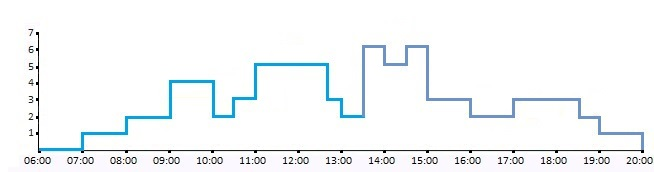
\includegraphics[width=1.0\textwidth]{reqshiftbreak1}
  \caption{The needed workers over planning period is shown with the blue line.}
  \label{fig:reqshiftbreak1} 
\end{figure}

\item  $shiftMinusRequirement_t : $ There are several shifts, that are characterized with start $s_i.start$ and length $s_i.length$ of shift $s_i$. First, we need to convert each shift $s_i$ with a number of workers $s_i.w_j$ in  each day $j$ to the number of people working in each time slot $t$. We need to calculate this working staff decreased by requirements of workers $shiftMinusRequirement_t$ in each time slot $t$ . In this calculation, we are not considering the breaks of workers. In Figure~\ref{fig:reqshiftbreak2} is shown an example graph with required employees and present employees (shifts without breaks). The breaks will fill these space between two curves, as it is shown in Figure~\ref{fig:reqshiftbreak3}.

\begin{equation}
shiftMinusRequirement_t \ge 0 \quad \forall t = 1, 2, ..., n
\end{equation}


\begin{figure}[h]
  \centering
  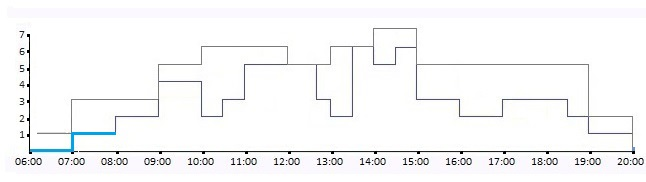
\includegraphics[width=1.0\textwidth]{reqshiftbreak2}
  \caption{Shifts are scheduled without breaks, The required workers (Blue Line) and present workers (Gray Line) are shown over planning period.}
  \label{fig:reqshiftbreak2} 
\end{figure}

\begin{figure}[h]
  \centering
  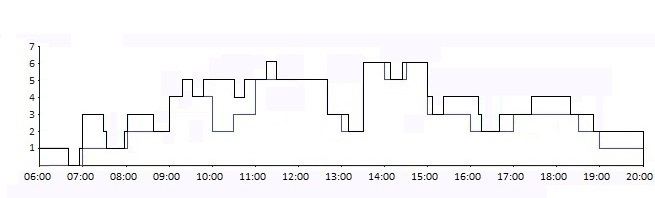
\includegraphics[width=1.0\textwidth]{reqshiftbreak3}
  \caption{ Breaks are assigned to each shift, The required employees (Blue Line) and working employees (Black Line) are shown over planning period.}
  \label{fig:reqshiftbreak3} 
\end{figure}


To calculate the number of workers in each time slot between these two curves, we use Algorithm~\ref{alg:convert-shifts}, is given above,

\begin{algorithm}
  \SetKw{BreakFor}{break for}
  \KwIn{$r_t$, $s_i.start$, $s_i.length$, $s_i.w_j$ }
  \KwOut{$shiftMinusRequirement_t$}
  \For{$t\leftarrow 0$ \KwTo n-1}
  {
    $shiftMinusRequirement_t = -  r_t$
  }
  \For{$i\leftarrow 0$ \KwTo Number of Shifts -1}
  {
     \For{$j\leftarrow 0$ \KwTo 6}
     {
        \For{$l\leftarrow 0$ \KwTo $s_i.length -1$}
        {
		 $shiftMinusRequirement[(s_i.start + l + n * j/7) \%n] += s_i.w_j$  ;
        }
     }
  }
  \Return{$shiftMinusRequirement_t$;}
  \caption{Convert Shift Schedules to the number of Assigned Workers in Each Time Slot}
  \label{alg:convert-shifts} 
\end{algorithm}


In the Algorithm~\ref{alg:convert-shifts}, first we set the $shiftMinusRequirement_t$ variable with the minus needed number of workers in each time slot $t$ (Line $2$).  The number of day cycle is considered $7$ days (a week) for break scheduling problem (Line $5$). Each day has $n/7$ time slots. Suppose that the $slotlength$ is equal to 5, time slots [0- 288) is the interval of the first day, second day is between [288, 576), .. , [1928, 0) is the interval of last day. 

The night shifts of last day continue to the beginning of the week, due to the cyclic structure. Therefore, we need to apply $\mod n$. In line $7$, the day number is converted to the first time slot of a day with $(n * j / 7) (\mod n)$ and we add the equation $s_i.start + l$  to calculate the each time slot $t$ belongs to the interval of shift $s_i$ on day $j$. The right side of the equation is equal to the number of employees in day $j$ and shift $s_i$. \\

\item As mentioned in \cite{li:2010:beer}, the common settings and the initialization of the used parameters in our formulation for the soft constraints $C0$ to $C6$ are given below (The weight constraints of soft constraints are initialised with $W_i \quad \forall i = \{ 0, 1, 2...6 \}$. ),

\begin{itemize}
\item $C_0 : $ The earliest start of the break $earliestStart$ is half an hour after the beginning of the shift and the latest end $latestEnd$ half an hour before the shift's end. The exception of this soft constraint is evaluated with the weight $W_0$ is 20. \\

\item $C_1 : $ The earliest start of the lunch break $lunchEarliestStart$ is $03:30$ hours and the latest end $lunchLatestEnd$ $06:00$ hours after the beginning of the shift. The weight value  $W_1$ of this constraint is equal to $10$. \\

\item $C_2 : $ Work periods are the durations of work between the breaks and also between the first break and start of a shift and the last break and end of a shift. These durations need to be between two parameters, that are the minimum length of work period $minWP$ and maximum length of work period $maxWP$. These parameters are set $00.30$ and $01:40$ and the weight value $W_2$ is equal to 20.  

Meanwhile, if the start time of the first break is before the earliest start and the end time of the last break is after the latest end, this situation violates two soft constraints, that are $C_0$ and $C_2$. \\

\item $C_3 : $ Employees need to have more break time $minBreakExceedsWorkLimit$, if they exceed a certain limit $workLimit$. This constraint is violated, after 50 minutes of the work period, have less than 20 minutes break and the weight value $W_3$ is equal to $20$.  \\

\item $C_4 : $ The break duration of employees needs not to be  less than 10 minutes ($minBreakLength$) and not more than one hour ($maxBreakLength$). The less and more break duration is evaluated with the weight, $W_4$ is 1. \\

\item $C_5 : $ Sum of the shortages of employees in each time interval during the planning period. The weight value  $W_5$ for each shortage is equal to $10$. \\

\item $C_6 : $ Sum of the excesses of employees in each time interval during the planning period. The weight value  $W_6$  for each excess is equal to $ 2$ .
\end{itemize}

Beer et. al in \cite{li:2010:beer} mentioned that in real world benchmarks, most of these constraints violations ($C_0$, $C_1$, $C_2$, $C_3$, $C_4$) are less than 5 percent for each instance, with respect to the weight values above. Therefore, we initialize our variables based on satisfying these first five constraints and evaluate the objective function with the remaining two soft constraints, that are excesses and shortages of workers in each time interval during the planning period. \\


\end{itemize}



\subsubsection{Decision Variables}

The proposed integer linear programming formulation for break scheduling problem, the decision variables are given below,

\subsubsection{Initialization of Breaks}

Each shift-day-duty $s$ have several breaks. We initialize these breaks with three types of break variables, based on different time windows $TW_i$ ($i = \{0,1,2 \}$ is the number of break type ). These three break types are $bl_{sbt}$, $l_{sbt}$, $al_{sbt}$.



In break scheduling problem, breaks can be assigned into time slot $t$ between the earliest start of the break $earliestStart$ and the latest end of the break $latestEnd$. Thus, $C_0$ constraint needs to be satisfied and the breaks must be into these intervals. These three break type variables are assigned true, if there exists a start of a break in the time slot $t$. 

\begin{equation}
bl_{sbt} = \left\{ \begin{array}{cc}
		1 & \mbox{if shift-day-duty $s$ have break $b$ before lunch, starts from time slot $t$} \\
		0 & \mbox{otherwise}
	    \end{array}
    \right.
\end{equation}

\begin{equation}
l_{st} = \left\{ \begin{array}{cc}
		1 & \mbox{if shift-day-duty $s$ have lunch break, starts from time slot $t$} \\
		0 & \mbox{otherwise}
	    \end{array}
    \right.
\end{equation}


\begin{equation}
al_{sbt} = \left\{ \begin{array}{cc}
		1 & \mbox{if shift-day-duty $s$ have break $b$ after lunch, starts from time slot $t$} \\
		0 & \mbox{otherwise}
	    \end{array}
    \right.
\end{equation}


These time slots are restricted with different time windows, based on types of breaks.  We are assuming that every staff has three monitor breaks before the lunch break and $m-4$ monitor breaks after the lunch break depends on $s_i.breakTime$ of shift $s_i$. We will present them as follows, and explain time windows in details:
\begin{itemize}

\item $bl_{sbt}$ : We assumed each shift-day-duty $s$ have three monitor breaks before lunch. We need to consider the followings to reduce the time window $TW_0$ (earliest and latest possible start) of this type of breaks, 


\begin{itemize}
\item[-] The earliest start of the before lunch breaks, based on constraint $C_0$, at  earliest start of the break $earliestStart$.
\item[-] These breaks are before the lunch break, therefore the latest start of a before lunch breaks can be the latest end of lunch break of a shift, based on constraint $C_1$. As an example with shift length 8 hours, the time window of before lunch break (Red) is illustrated below, \\

\begin{tikzpicture}

%draw horizontal line
\draw (0,0.2) rectangle (12,-0.2);

%draw vertical lines
\foreach \x in {0,0.75,9,11.25,12}
\draw (\x cm,5.5pt) -- (\x cm,-5.5pt);



\draw (0,0) node[above=5.5pt] {$ 0 $} node[below=5.5pt] {$ Start  $};
\draw (0.75,0) node[above=5.5pt] {$ 6 $};

\draw (5.25,0) node[above=5.5pt] {$ 42 $};
\draw (9,0) node[above=5.5pt] {$ 72 $};

\draw (11.25,0) node[above=5.5pt] {$ 90 $};
\draw (12,0) node[above=5.5pt] {$ 96 $} node[below=5.5pt] {$ End $};

\draw[line width=11pt, color=red] (0.76,0) rectangle (9, 0)[above=3pt];
\end{tikzpicture}


\item[-] We can still restrict the time window $TW_0$. We need to consider that employees have a lunch break after these breaks and before the latest end of lunch break. The employees can have their lunch break as latest in the end of the lunch break period (last 6 time slots) and before the lunch break, the staff must work minimum 6 time slots ($minWP$), due to the constraint $C_2$. 

\item[-] The monitor break variables have length of 2 time slots. Consider time slot $t$ is the start time of the break, we need to decrease 2 more time slots from the latest start of the before lunch breaks. The illustrated example of the restricted time window of before lunch break with shift length 8 is shown below (Red: Time Window of Before Lunch Break, Black: Monitor Break, Yellow: Minimum Working Period, Blue: Lunch Break), \\

\begin{tikzpicture}

%draw horizontal line
\draw (0,0.2) rectangle (12,-0.2);

%draw vertical lines
\foreach \x in {0,0.75,9,11.25,12}
\draw (\x cm,5.5pt) -- (\x cm,-5.5pt);



\draw (0,0) node[above=5.5pt] {$ 0 $} node[below=5.5pt] {$ Start  $};
\draw (0.75,0) node[above=5.5pt] {$ 6 $};

\draw (5.25,0) node[above=5.5pt] {$ 42 $};
\draw (7.15,0) node[above=5.5pt] {$ 58 $};
\draw (7.6,0) node[above=5.5pt] {$ 60 $};
\draw (8.25,0) node[above=5.5pt] {$ 66 $};
\draw (9,0) node[above=5.5pt] {$ 72 $};

\draw (11.25,0) node[above=5.5pt] {$ 90 $};
\draw (12,0) node[above=5.5pt] {$ 96 $} node[below=5.5pt] {$ End $};

\draw[line width=11pt, color=red] (0.76,0) rectangle (7.25, 0)[above=3pt];
\draw[line width=11pt, color=black] (7.25,0) rectangle (7.5, 0)[above=3pt];
\draw[line width=11pt, color=yellow] (7.5,0) rectangle (8.25, 0)[above=3pt];
\draw[line width=11pt, color=blue] (8.25,0) rectangle (9, 0)[above=3pt];

\end{tikzpicture}
\end{itemize}

From the restrictions above, the time window of before lunch breaks is calculated below,

\begin{equation}
es_0  = earliestStart
\end{equation}

\begin{equation}
ls_0 = lunchLatestEnd - lunchBreakTime- minWP -2
\end{equation}

The time windows of these three breaks are also tightened between each other from the following statements,

\begin{itemize}
\item[-]  The earliest start of the first before lunch break is the earliest start of the break $earliestStart$. However, it must end before the other remaining two before lunch breaks. Therefore, we consider the last before lunch break starts at the latest start of the time window above. Before this break the employee need to work $minWP$. The second break finishes at latest at this point of time. Therefore, if we decrease 2 time slots (length of second break) and $minWP$ (between the first and second break), we can find the latest point of the end of the first break. At last, we need to decrease 2 more time slot to find the latest start of the first before lunch break. The illustrated example  of the restricted time window for the first before lunch break is given below (Red : Time Window of Before Lunch Break, Black: Monitor Break, Yellow: Minimum Working Period, Blue: Lunch Break), \\


\begin{tikzpicture}
%draw horizontal line
\draw (0,0.2) rectangle (12,-0.2);

%draw vertical lines
\foreach \x in {0,0.75,9,11.25,12}
\draw (\x cm,5.5pt) -- (\x cm,-5.5pt);

\draw (0,0) node[above=5.5pt] {$ 0 $} node[below=5.5pt] {$ Start  $};
\draw (0.75,0) node[above=5.5pt] {$ 6 $};

\draw (5.15,0) node[above=5.5pt] {$ 42 $};
\draw (5.6,0) node[above=5.5pt] {$ 44 $};
\draw (6.15,0) node[above=5.5pt] {$ 50 $};
\draw (6.6,0) node[above=5.5pt] {$ 52 $};
\draw (7.15,0) node[above=5.5pt] {$ 58 $};
\draw (7.6,0) node[above=5.5pt] {$ 60 $};
\draw (8.25,0) node[above=5.5pt] {$ 66 $};
\draw (9,0) node[above=5.5pt] {$ 72 $};

\draw (11.25,0) node[above=5.5pt] {$ 90 $};
\draw (12,0) node[above=5.5pt] {$ 96 $} node[below=5.5pt] {$ End $};

\draw[line width=11pt, color=red] (0.76,0) rectangle (5.25, 0)[above=3pt];
\draw[line width=11pt, color=black] (5.25,0) rectangle (5.5, 0)[above=3pt];
\draw[line width=11pt, color=yellow] (5.5,0) rectangle (6.25, 0)[above=3pt];
\draw[line width=11pt, color=black] (6.25,0) rectangle (6.5, 0)[above=3pt];
\draw[line width=11pt, color=yellow] (6.5,0) rectangle (7.25, 0)[above=3pt];
\draw[line width=11pt, color=black] (7.25,0) rectangle (7.5, 0)[above=3pt];
\draw[line width=11pt, color=yellow] (7.5,0) rectangle (8.25, 0)[above=3pt];
\draw[line width=11pt, color=blue] (8.25,0) rectangle (9, 0)[above=3pt];


\end{tikzpicture}
\item[-] We have already calculated the latest start of the second break, that is $minWP + 2$ time slots before the old latest start. The earliest start of the second before lunch break must be after the first break, therefore, we need to add to the first before lunch break, $minWP + 2$ time slots, to the earliest start of the break. As an example of the restricted time window for the second before lunch break is shown below (Red : Time Window of Before Lunch Break, Black : Monitor Break, Yellow : Minimum Working Period, Blue : Lunch Break), \\


\begin{tikzpicture}
%draw horizontal line
\draw (0,0.2) rectangle (12,-0.2);

%draw vertical lines
\foreach \x in {0,0.75,9,11.25,12}
\draw (\x cm,5.5pt) -- (\x cm,-5.5pt);



\draw (0,0) node[above=5.5pt] {$ 0 $} node[below=5.5pt] {$ Start  $};
\draw (0.65,0) node[above=5.5pt] {$ 6 $};
\draw (1.1,0) node[above=5.5pt] {$ 8 $};
\draw (1.75,0) node[above=5.5pt] {$ 14 $};
\draw (6.15,0) node[above=5.5pt] {$ 50 $};
\draw (6.6,0) node[above=5.5pt] {$ 52 $};
\draw (7.15,0) node[above=5.5pt] {$ 58 $};
\draw (7.6,0) node[above=5.5pt] {$ 60 $};
\draw (8.25,0) node[above=5.5pt] {$ 66 $};
\draw (9,0) node[above=5.5pt] {$ 72 $};

\draw (11.25,0) node[above=5.5pt] {$ 90 $};
\draw (12,0) node[above=5.5pt] {$ 96 $} node[below=5.5pt] {$ End $};

\draw[line width=11pt, color=black] (0.76,0) rectangle (1.0, 0)[above=3pt];
\draw[line width=11pt, color=yellow] (1.0,0) rectangle (1.75, 0)[above=3pt];
\draw[line width=11pt, color=red] (1.75,0) rectangle (6.25, 0)[above=3pt];
\draw[line width=11pt, color=black] (6.25,0) rectangle (6.5, 0)[above=3pt];
\draw[line width=11pt, color=yellow] (6.5,0) rectangle (7.25, 0)[above=3pt];
\draw[line width=11pt, color=black] (7.25,0) rectangle (7.5, 0)[above=3pt];
\draw[line width=11pt, color=yellow] (7.5,0) rectangle (8.25, 0)[above=3pt];
\draw[line width=11pt, color=blue] (8.25,0) rectangle (9, 0)[above=3pt];


\end{tikzpicture}
\item[-] With the same rule, the third before lunch break must start after $2 *  (minWP + 2)$ from earliest start of the break and latest start is the old latest start, that we calculated above. The illustrated example  of the restricted time window for the last before lunch break is given below (Red : Time Window of Before Lunch Break, Black : Monitor Break, Yellow : Minimum Working Period, Blue : Lunch Break), \\


\begin{tikzpicture}

%draw horizontal line
\draw (0,0.2) rectangle (12,-0.2);

%draw vertical lines
\foreach \x in {0,0.75,9,11.25,12}
\draw (\x cm,5.5pt) -- (\x cm,-5.5pt);



\draw (0,0) node[above=5.5pt] {$ 0 $} node[below=5.5pt] {$ Start  $};
\draw (0.65,0) node[above=5.5pt] {$ 6 $};
\draw (1.1,0) node[above=5.5pt] {$ 8 $};
\draw (1.65,0) node[above=5.5pt] {$ 14 $};
\draw (2.1,0) node[above=5.5pt] {$ 16 $};
\draw (2.75,0) node[above=5.5pt] {$ 22 $};
\draw (7.15,0) node[above=5.5pt] {$ 58 $};
\draw (7.6,0) node[above=5.5pt] {$ 60 $};
\draw (8.25,0) node[above=5.5pt] {$ 66 $};
\draw (9,0) node[above=5.5pt] {$ 72 $};

\draw (11.25,0) node[above=5.5pt] {$ 90 $};
\draw (12,0) node[above=5.5pt] {$ 96 $} node[below=5.5pt] {$ End $};

\draw[line width=11pt, color=black] (0.76,0) rectangle (1.0, 0)[above=3pt];
\draw[line width=11pt, color=yellow] (1.0,0) rectangle (1.75, 0)[above=3pt];
\draw[line width=11pt, color=black] (1.75,0) rectangle (2.0, 0)[above=3pt];
\draw[line width=11pt, color=yellow] (2.0,0) rectangle (2.75, 0)[above=3pt];
\draw[line width=11pt, color=red] (2.75,0) rectangle (7.25, 0)[above=3pt];
\draw[line width=11pt, color=black] (7.25,0) rectangle (7.5, 0)[above=3pt];
\draw[line width=11pt, color=yellow] (7.5,0) rectangle (8.25, 0)[above=3pt];
\draw[line width=11pt, color=blue] (8.25,0) rectangle (9, 0)[above=3pt];

\end{tikzpicture}
\end{itemize}


As a summary, we added $i * ( minWP +2 )$ to the earliest start of a break and decrease $(2 - i) * ( minWP +2 )$ from the latest start where $i$ indicating the number of before lunch break -1. The updated interval of time window $TW_0$ of before lunch break is given below,

\begin{equation}
es_0  = earliestStart + i * ( minWP +2 ) 
\end{equation}

\begin{equation}
ls_0 = lunchLatestEnd - lunchBreakTime-  (3 - i) * ( minWP + 2 ) 
\end{equation}
\begin{equation}
 \forall i = \{0,1,2\}
\end{equation}


\item $l_{st}$ : The shifts have at most one lunch break, therefore this variable is initialized with two dimensions shift-day-duty $s$ and time slot $t$. The lunch break can be between the Lunch Earliest Start and Lunch Latest End - Lunch Break Time. This break has length 6 time slots. The illustration of time window $TW_1$  of lunch break is shown below, (Blue: Time Window of Lunch Break, Black: Lunch Break), \\

\begin{tikzpicture}

%draw horizontal line
\draw (0,0.2) rectangle (12,-0.2);

%draw vertical lines
\foreach \x in {0,0.75,5.25,9,11.25,12}
\draw (\x cm,5.5pt) -- (\x cm,-5.5pt);

\draw (0,0) node[above=5.5pt] {$ 0 $} node[below=5.5pt] {$ Start  $};
\draw (0.75,0) node[above=5.5pt] {$ 6 $};

\draw (5.25,0) node[above=5.5pt] {$ 42 $};
\draw (9,0) node[above=5.5pt] {$ 72 $};


\draw (12,0) node[above=5.5pt] {$ Shift Duration $} node[below=5.5pt] {$ End $};


\draw[line width=11pt, color=blue] (5.26, 0) rectangle (8.25, 0)[above=3pt];
\draw[line width=11pt, color=black] (8.25,0) rectangle (9, 0)[above=3pt];
\end{tikzpicture}

The earliest start and latest start of a lunch break is given below,

\begin{equation}
es_1 =  Lunch Earliest Start 
\end{equation}

\begin{equation}
ls_1 =  Lunch Latest End - Lunch Break Time
\end{equation}

\item $al_{sbt}$ : We assumed each shift-day-duty $s$ have $m-4$ monitor breaks after lunch, based on length of the shift. We need to consider the followings to calculate the time window $TW_2$ of these types of breaks, 

\begin{itemize}

\item[-] The latest start of the after lunch breaks, based on constraint $C_0$, at  latest end of the break $latestEnd$. 

\item[-] These breaks are after the lunch break, therefore the earliest start can be the  earliest start of lunch break of a shift. As an example with shift length 8 hours, the time window of after lunch break (Green) is illustrated below, \\

\begin{tikzpicture}

%draw horizontal line
\draw (0,0.2) rectangle (12,-0.2);

%draw vertical lines
\foreach \x in {0,0.75,5.25,9,11.25,12}
\draw (\x cm,5.5pt) -- (\x cm,-5.5pt);

\draw (0,0) node[above=5.5pt] {$ 0 $} node[below=5.5pt] {$ Start  $};
\draw (0.75,0) node[above=5.5pt] {$ 6 $};

\draw (5.25,0) node[above=5.5pt] {$ 42 $};
\draw (9,0) node[above=5.5pt] {$ 72 $};

\draw (11.25,0) node[above=5.5pt] {$ 90 $};
\draw (12,0) node[above=5.5pt] {$ 96 $} node[below=5.5pt] {$ End $};

\draw[line width=11pt, color=green] (5.26, 0) rectangle (11.25, 0)[above=3pt];
\end{tikzpicture}


\item[-] Likewise, in before lunch break, we can also reduce the time window $TW_2$ of after lunch break. We need to consider that employees have a lunch break before these breaks. Therefore, assuming the employees have lunch break in the beginning of the lunch break period (first 6 time slot) and after the lunch, the staff must have a working period minimum 6 time slots, due to the constraint $C_2$. 

\item[-]  The monitor break variables have a length of 2 time slots. Consider time slot $t$ is the start time of the break, we need to decrease 2 time slot from the latest end of the break  $latestEnd$. The illustrated example of the restricted time window of after lunch break with shift length 8 is shown below (Green : Time Window of After Lunch Break, Black : Monitor Break, Yellow : Minimum Working Period, Blue : Lunch Break), \\


\begin{tikzpicture}

%draw horizontal line
\draw (0,0.2) rectangle (12,-0.2);

%draw vertical lines
\foreach \x in {0,0.75,9,11.25,12}
\draw (\x cm,5.5pt) -- (\x cm,-5.5pt);



\draw (0,0) node[above=5.5pt] {$ 0 $} node[below=5.5pt] {$ Start  $};
\draw (0.75,0) node[above=5.5pt] {$ 6 $};

\draw (5.25,0) node[above=5.5pt] {$ 42 $};
\draw (6,0) node[above=5.5pt] {$ 48 $};
\draw (6.75,0) node[above=5.5pt] {$ 54 $};
\draw (8.25,0) node[above=5.5pt] {$ 72 $};
\draw (10.9,0) node[above=5.5pt] {$ 88 $};

\draw (11.35,0) node[above=5.5pt] {$ 90 $};
\draw (12,0) node[above=5.5pt] {$ 96 $} node[below=5.5pt] {$ End $};

\draw[line width=11pt, color=blue] (5.26,0) rectangle (6, 0)[above=3pt];
\draw[line width=11pt, color=yellow] (6,0) rectangle (6.75, 0)[above=3pt];
\draw[line width=11pt, color=green] (6.75, 0) rectangle (11.00, 0)[above=3pt];
\draw[line width=11pt, color=black] (11.00, 0) rectangle (11.25, 0)[above=3pt];
\end{tikzpicture}
\end{itemize}

As we explained in before lunch breaks, we can also restrict the time window of each after lunch break $TW_2$ between each other. We add i * ( minWP +2 ) to earliest start of after lunch break and decrease  (m - 5- i) * ( minWP +2 ) from latest start of after lunch break where $i$ indicating the number of after lunch break -1. From the all restrictions above, the earliest and latest start of after lunch breaks are calculated as given below,

\begin{equation}
es_2 = Lunch Earliest Start + Lunch Break Time + minWP * ( i +1) +2 i  
\end{equation}

\begin{equation}
ls_2 = Latest End - 2 - (m - 5 -  i) *  (2 +  minWP)  
\end{equation}

\begin{equation}
\forall i = \{0,1, .. , m-5\}
\end{equation}


The illustrated example of the restricted time window for the first after lunch break with shift length 8 is given below (Green: Time Window of After Lunch Break, Black: Monitor Break, Yellow: Minimum Working Period, Blue: Lunch Break), \\

\begin{tikzpicture}
%draw horizontal line
\draw (0,0.2) rectangle (12,-0.2);

%draw vertical lines
\foreach \x in {0,0.75,9,11.25,12}
\draw (\x cm,5.5pt) -- (\x cm,-5.5pt);

\draw (0,0) node[above=5.5pt] {$ 0 $} node[below=5.5pt] {$ Start  $};
\draw (0.75,0) node[above=5.5pt] {$ 6 $};

\draw (5.25,0) node[above=5.5pt] {$ 42 $};
\draw (6,0) node[above=5.5pt] {$ 48 $};
\draw (6.75,0) node[above=5.5pt] {$ 54 $};
\draw (8.9,0) node[above=5.5pt] {$ 72 $};
\draw (9.35,0) node[above=5.5pt] {$ 74 $};
\draw (9.9,0) node[above=5.5pt] {$80 $};
\draw (10.35,0) node[above=5.5pt] {$ 82 $};
\draw (10.9,0) node[above=5.5pt] {$ 88 $};
\draw (11.35,0) node[above=5.5pt] {$ 90 $};
\draw (12,0) node[above=5.5pt] {$ 96 $} node[below=5.5pt] {$ End $};


\draw[line width=11pt, color=blue] (5.26,0) rectangle (6, 0)[above=3pt];
\draw[line width=11pt, color=yellow] (6,0) rectangle (6.75, 0)[above=3pt];
\draw[line width=11pt, color=green] (6.75, 0) rectangle (9.00, 0)[above=3pt];
\draw[line width=11pt, color=black] (9,0) rectangle (9.25, 0)[above=3pt];
\draw[line width=11pt, color=yellow] (9.25,0) rectangle (10, 0)[above=3pt];
\draw[line width=11pt, color=black] (10,0) rectangle (10.25, 0)[above=3pt];
\draw[line width=11pt, color=yellow] (10.25,0) rectangle (11, 0)[above=3pt];
\draw[line width=11pt, color=black] (11.00, 0) rectangle (11.25, 0)[above=3pt];

\end{tikzpicture}

The second after lunch break  with shift length 8 is shown below (Green: Time Window of After Lunch Break, Black: Monitor Break, Yellow: Minimum Working Period, Blue: Lunch Break), \\


\begin{tikzpicture}
%draw horizontal line
\draw (0,0.2) rectangle (12,-0.2);

%draw vertical lines
\foreach \x in {0,0.75,9,11.25,12}
\draw (\x cm,5.5pt) -- (\x cm,-5.5pt);




\draw (0,0) node[above=5.5pt] {$ 0 $} node[below=5.5pt] {$ Start  $};
\draw (0.75,0) node[above=5.5pt] {$ 6 $};

\draw (5.25,0) node[above=5.5pt] {$ 42 $};
\draw (6,0) node[above=5.5pt] {$ 48 $};
\draw (6.65,0) node[above=5.5pt] {$ 54 $};
\draw (7.1,0) node[above=5.5pt] {$ 56 $};
\draw (7.75,0) node[above=5.5pt] {$ 62 $};
\draw (9.9,0) node[above=5.5pt] {$80 $};
\draw (10.35,0) node[above=5.5pt] {$ 82 $};
\draw (10.9,0) node[above=5.5pt] {$ 88 $};
\draw (11.35,0) node[above=5.5pt] {$ 90 $};
\draw (12,0) node[above=5.5pt] {$ 96 $} node[below=5.5pt] {$ End $};

\draw[line width=11pt, color=blue] (5.26,0) rectangle (6, 0)[above=3pt];
\draw[line width=11pt, color=yellow] (6,0) rectangle (6.75, 0)[above=3pt];
\draw[line width=11pt, color=black] (6.75,0) rectangle (7, 0)[above=3pt];
\draw[line width=11pt, color=yellow] (7,0) rectangle (7.75, 0)[above=3pt];
\draw[line width=11pt, color=green] (7.75, 0) rectangle (10.00, 0)[above=3pt];
\draw[line width=11pt, color=black] (10,0) rectangle (10.25, 0)[above=3pt];
\draw[line width=11pt, color=yellow] (10.25,0) rectangle (11, 0)[above=3pt];
\draw[line width=11pt, color=black] (11.00, 0) rectangle (11.25, 0)[above=3pt];


\end{tikzpicture}

The illustrated example  of the restricted time window for the last after lunch break  with shift length 8 is given below (Green: Time Window of After Lunch Break, Black: Monitor Break, Yellow: Minimum Working Period, Blue: Lunch Break), \\


\begin{tikzpicture}

%draw horizontal line
\draw (0,0.2) rectangle (12,-0.2);

%draw vertical lines
\foreach \x in {0,0.75,9,11.25,12}
\draw (\x cm,5.5pt) -- (\x cm,-5.5pt);

\draw (0,0) node[above=5.5pt] {$ 0 $} node[below=5.5pt] {$ Start  $};
\draw (0.75,0) node[above=5.5pt] {$ 6 $};

\draw (5.25,0) node[above=5.5pt] {$ 42 $};
\draw (6,0) node[above=5.5pt] {$ 48 $};
\draw (6.65,0) node[above=5.5pt] {$ 54 $};
\draw (7.1,0) node[above=5.5pt] {$ 56 $};
\draw (7.65,0) node[above=5.5pt] {$ 62 $};
\draw (8.1,0) node[above=5.5pt] {$64 $};
\draw (8.75,0) node[above=5.5pt] {$ 70 $};
\draw (10.9,0) node[above=5.5pt] {$ 88 $};
\draw (11.35,0) node[above=5.5pt] {$ 90 $};
\draw (12,0) node[above=5.5pt] {$ 96 $} node[below=5.5pt] {$ End $};

\draw[line width=11pt, color=blue] (5.26,0) rectangle (6, 0)[above=3pt];
\draw[line width=11pt, color=yellow] (6,0) rectangle (6.75, 0)[above=3pt];
\draw[line width=11pt, color=black] (6.75,0) rectangle (7, 0)[above=3pt];
\draw[line width=11pt, color=yellow] (7,0) rectangle (7.75, 0)[above=3pt];
\draw[line width=11pt, color=black] (7.75,0) rectangle (8, 0)[above=3pt];
\draw[line width=11pt, color=yellow] (8,0) rectangle (8.75, 0)[above=3pt];
\draw[line width=11pt, color=green] (8.75, 0) rectangle (11.00, 0)[above=3pt];
\draw[line width=11pt, color=black] (11.00, 0) rectangle (11.25, 0)[above=3pt];

\end{tikzpicture}








\end{itemize}























\begin{itemize}

\item $st_{sb}$ : Start time is an integer positive variable, indicating the time slot of the start of the breaks within their shift. Every break $b$ of shift-day-duty $s$ have a start time and the value of start time is between this interval below, 


\begin{equation}
 0 \le st_{sb} \le  Shift Length -Earliest Start -Latest End - 2  
\end{equation} 
\begin{equation}
\forall s = \{0, 1 ...sdd -1\} \quad \forall b = \{0, 1, ...,m -1 \}
\end{equation} 

We needed the start time of each break to calculate work period between each other. The equation to calculate the start time will be explained in constraint section.




\item $wp_{sb}$ : There are two soft constraints based on a work period in the problem statement, however, as we mentioned before, we added this constraint directly to our initialization of the problem. $wp_{sb}$ is defined as follows,

\begin{itemize}
\item  The duration from the start time of the shift to the beginning of first break.
\item  The duration from the end time of  each break to the start time of the following break belongs to the same shift-day-duty.
\item  The duration from the end of the last break to the end of the shift.
\end{itemize}

We initialize the work period $wp_{sb}$  variable, based on start time $st_{sb}$ in the constraint section more clearly. This variable must be due to constraint $C_2$ between the interval [00:30, 01:40].

Based on the constraint $C_3$, if an employee exceeds 50 minute work period, he must have 20 minutes break. Each monitor break has 10 minutes length. Therefore, we initialize each work period have between 30 minutes to 50 minutes long, except two working periods. These two working periods are,

\begin{itemize}
\item The working period before the lunch break, because the lunch break is 30 minutes long, therefore the employee can exceed 50 minutes working period before. \\
\item The working period after the last break. Because, the employee will finish his duty and will be free.
\end{itemize}


We initialize the each working period between interval, 

\begin{equation}
00:30 \le wp_{sb} \le 01:40 \quad \forall s = \{0, 1 ...sdd -1\} \quad \forall b = \{0, 1, ..., m\}
\end{equation} 

We add the constraint whether working period is less or equal to 50 minutes or not in the following section. 

\item We added first five soft constraints into our formulation as an hard constraint. The remaining two components of the objective function are :
\begin{itemize}
\item $C_5$ : Sum of excesses of employees in each time slot. 

\item $C_6$ : Sum of shortages of employees in each time slot. \\
\end{itemize} 

\item To calculate these two components, we needed two variables $ex_t$, $sh_t$ like in shift design problem, 
\begin{itemize}
\item $ex_t$ : Excesses  of workers in time slot $t$.

\item $sh_t$ : Shortages of workers in time slot $t$. \\
\end{itemize}
\end{itemize}

\subsection{Constraints}
We will present the constraints, we use in our integer programming formulation in 2 sections, soft and hard constraints. 


\subsubsection{Hard Constraints}

\begin{itemize}
\item Each break of shift-day-duty $s$ must assign to exactly one time slot $t$. For each break type the equations are shown below,

\begin{itemize}
\item For before lunch breaks $bl_{sbt}$,


\begin{equation}
\sum_{t \in TW_0 } bl_{sbt} = 1 \quad \forall s = \{0, 1, ..., sdd -1\} \quad  \forall b = \{0, 1, 2\}
\end{equation}

\item For lunch breaks $l_{st}$,

\begin{equation}
\sum_{t \in TW_1} l_{st} = 1 \quad \forall s = \{0, 1, ...,sdd -1\} 
\end{equation}

\item For after lunch breaks $al_{sbt}$,

\begin{equation}
\sum_{t \in TW_2} al_{sbt} = 1 \quad  \forall s = \{0, 1, ...,sdd -1\} \quad \forall b = \{0, 1, ...,m - 4\}
\end{equation}


\end{itemize} 



\item $st_{sb} : $ Start time variable indicates the time difference between the break $b$ start and the belonging shift start $s_i.start$. The start times of each break are initialized based on each break type, are given below,


\begin{itemize}
\item  The dimension $t$ in variable $bl_{sbt}$, represent the start point of a break after the earliest start of before lunch breaks. We calculate the earliest start of the before lunch breaks $es_0$ as Earliest Start +$ (minWP + 2) * i$, where $i$ is indicating the number of before lunch break. $st_{sb}$ is initialized for each before lunch break as follows,

\begin{equation}
st_{sb} =es_0 + t * bl_{sbt} \quad \forall s = \{0, 1 ...sdd -1\} \quad \forall t \in TW_0 \quad \forall b = \{0, 1, 2\}
\end{equation}

\item There is just one lunch break and it is the fourth break (b = 3). The earliest start of the lunch break $es_1$ is lunch earliest start. The initialization of it, is given below,

\begin{equation}
st_{s3} =  es_1 + t * l_{st} \quad \forall s = \{0, 1 ...sdd -1\} \quad \forall t \in TW_1
\end{equation}

\item The earliest start of the after lunch breaks  $es_2$ is  initialized as Lunch Earliest Start + Lunch Break Time + $minWP + (minWP + 2) * i$ where $i$ is representing the number of after lunch break. The start times of first 4 breaks are initialized before, therefore we add 4 to the value of $b$ to initialize start time of after lunch breaks.

\begin{equation}
st_{s(b+4)} =es_2 + t * al_{sbt}  \quad \forall s = \{0, 1 ...sdd -1\} \quad \forall t \in  TW_2 \quad \forall b = \{0, 1, .., m-5\}
\end{equation}

\end{itemize}


\item $wp_{sb} : $ We add the constraint $C_2$ and $C_3$ into our formulation in this section. The end time of each break is the addition of  start time and break duration (Monitor breaks : 2 time slots, Lunch breaks : 6 time slots). Therefore, for these constraints, the work period is initialized based on start time and duration of each break. The equations to calculate work periods are given below,

\begin{itemize}
\item The first work period is equal to the start time of the first break, because the start time variable is the length from the shift start. 

\begin{equation}
wp_{s0} = st_{s0} \quad \forall s = \{0, 1 ...sdd -1\}
\end{equation}

\item The last work period is equal to the equation given below,

\begin{equation}
wp_{sm} = Shift Length - st_{s(m-1)} - 2 \quad \forall s = \{0, 1 ...sdd -1\}
\end{equation}

\item The work periods of the remaining breaks are between the end of the break and start of the following break. Therefore, they are initialized as follows,


\begin{equation}
wp_{sb} = st_{sb} - st_{s(b-1)}  -2 \quad \forall s = \{0, 1 ...sdd -1\} \quad \forall b = \{1,2.., m-1\}
\end{equation}

\end{itemize}

The work period variable is already initialized between the interval [00:30, 01:40], due to constraint $C_2$. We need to decrease the length of the work period to $workLimit$ (50 minutes) based on constraint $C_3$, if the following break is shorter than 20 minutes ($minBreakExceedsWorkLimit$). The work period before lunch (b=2) and the last work period (b=m) can be more than 50 minutes. Therefore, we add constraints below,

\begin{equation}
wp_{sb} \le workLimit \quad \forall s = \{0, 1 ...sdd -1\} \quad \forall b = \{0, 1, 3, .., m-1\}
\end{equation}

\end{itemize}

\subsubsection{Soft  Constraints}

As we mentioned before, the objective function consists of two remaining soft constraints ($C_5, C_6$) , these are excesses and shortages of employees in each time slot. To find these components, we use the $shiftMinusRequirement_t$ variable, that represent the number of employees remaining after we reduced the required employee of each time slot from the working employees (without considering breaks) belongs to all shifts. 

In this part, we will include the breaks of employees and decrease from the variable $shiftMinusRequirement_t$ to the employees, that are at lunch or monitor breaks belongs to each shift-day-duty in each time slot. The result of this equation can be in each time slot,
\begin{itemize}
\item 0 : There are not any excesses or shortages of workers in time slot $t$. 
\item Positive : There are excesses of workers $ex_t$ in time slot $t$. 
\item Negative : There are shortages of workers $sh_t$ in time slot $t$. 
\end{itemize}



The same as in shift design problem, we calculate the excesses and shortages of employees in time slot $t$ with the equation, is given below,

\begin{equation}
breaks_t - sh_t + ex_t = shiftMinusRequirement_t \quad \forall t = \{0, 1, 2, .., n-1\}
\end{equation}

where,
\begin{itemize}
\item[]  $breaks_t : $ Sum of employees have break in time slot $t$ 
\item[]  $ex_t : $ This variable is a positive integer and the positive value of the equation $shiftMinusRequirement_t - breaks_t$
is equal to excesses  $ex_t$  of employees in time slot $t$.
\item[]  $sh_t : $ This variable is a positive integer and the negative value of  the equation $shiftMinusRequirement_t - breaks_t$
is equal to shortages  $sh_t$ of employees in time slot $t$.
\end{itemize}

We need to calculate the $breaks_t$ variable, that is the sum of all employees in before lunch, lunch or after lunch breaks in time slot $t$ in planning period (t =\{0,1, ...,n\}). The illustration of calculation $breaks_t$ variable and the excesses $ex_t$ and shortages $sh_t$ of employees in time slot $t$ is given in Algorithm~\ref{alg:excesses-shortages}. This variable is calculated based on 2 statements, are given below,
\begin{itemize}

\item We initialized the before lunch breaks, lunch break or after lunch breaks based on time window of belonging shift-day-duty $s$ and time slot $t$ is the start time value of break between the time window of each break type. We need to convert this $t$ value to a general time slot in planning period (0,1, ...,n). For each break type the calculation is different, based on different time window. 


\item Each monitor break, before lunch breaks and after lunch breaks, is 2 time slots and a staff needs a full time slot to continue his work after his each break. This time slot is considered neither break, nor work period. However, we need to add these full time slot also to $breaks_t$ variable to calculate excesses and shortages of workers. In total monitor breaks need to be considered as 3 time slots and with this extra time slot, lunch breaks have 7 time slot length.

\end{itemize}

\begin{algorithm}
  \SetKw{BreakFor}{break for}
  \KwIn{$bl_{sbt}$, $l_{st}$, $al_{sbt}$, $s_i.start$, $shiftMinusRequirement_t$ .. }
  \KwOut{$sh_t, ex_t$}
  \For{$i\leftarrow 0$ \KwTo $n-1$}
  {
     \For{$s\leftarrow 0$ \KwTo $sdd - 1$}
     {
        \For{$t \in TW_0$}
        {
           \For{$b\leftarrow 0$ \KwTo $2$}
           {
              \If{$i = (t + s_i.start + earliestStart + (minWP + 2) * b + (daySDD.get(s) * n / 7)) \mod n$}
              {
		 $breaks_i += bl_{sbt} + bl_{sb(t-1)} + bl_{sb(t-2)}$  ;
              }
           }
        }

        \For{$t \in TW_1$}
        {
           \If{$i = (t + s_i.start + lunchEarliestStart + (daySDD.get(s) * n / 7)) \mod n$}
           {
              \For{$j\leftarrow 0$ \KwTo $6$}
              {
		 $breaks_i += l_{s(t-j)}$  ;
              }
           }
        }

        \For{$t \in TW_2$}
        {
           \For{$b\leftarrow 0$ \KwTo $m-5$}
           {
              \If{$i = (t + s_i.start + lunchEarliestStart + 6  + minWP + (minWP + 2) * b + (daySDD.get(s) * n / 7)) \mod n$}
              {
		 $breaks_i += al_{sbt} + al_{sb(t-1)} + al_{sb(t-2)}$  ;
              }
           }
        }
   }
   $breaks_i - sh_i + ex_i = shiftMinusRequirement_i$ ;
}
  \Return{$ sh_t,  ex_t $;}
  \caption{Algorithm to calculate sum of all employees have break in time slot $t$}
  \label{alg:excesses-shortages} 
\end{algorithm}

In Algorithm~\ref{alg:excesses-shortages} , we use if statements (5. - 11. - 19. Lines) to get each type of breaks from the general time slot $i$ in planning period ($i = \{0,1,... n-1\}$) . Each calculation is different based on earliest start $es_0$ (Line 5), $es_1$  (Line 11), $es_2$ (Line 19) of break types. $\mod n$ is used, due to the cyclic structure and the day number is converted to the first time slot of a day with $(daySDD.get(s) * n / 7) (\mod n)$. In Line 6 - 13 - 20, we calculate the sum of employees of each break type based on duration of breaks. \\

Sum of excesses/ shortages of workers in each time slot is calculated,

\begin{itemize}
\item Sum of excesses of employees in each time slot 
\begin{equation}
C_5 = \sum_{t=0}^{n-1} ex_t
\end{equation}
\item Sum of shortages of employees in each time slot

\begin{equation}
C_6 = \sum_{t=0}^{n-1} sh_t
\end{equation}
\end{itemize}



\subsection{Objective function}
The objective function is combined two remaining weighted criteria

\begin{equation}
\min \sum_{i=5}^6 W_i * C_i
\end{equation}


 

\chapter{Computational Experiments}
%% intro.tex
%% Copyright (C) 2014 by Thomas Auzinger <thomas.auzinger@cg.tuwien.ac.at>
%
% This work may be distributed and/or modified under the
% conditions of the LaTeX Project Public License, either version 1.3
% of this license or (at your option) any later version.
% The latest version of this license is in
%   http://www.latex-project.org/lppl.txt
% and version 1.3 or later is part of all distributions of LaTeX
% version 2005/12/01 or later.
%
% This work has the LPPL maintenance status `maintained'.
%
% The Current Maintainer of this work is Thomas Auzinger.
%
% This work consists of the files vutinfth.dtx and vutinfth.ins
% and the derived file vutinfth.cls.
% This work also consists of the file intro.tex.


\newacronym{ctan}{CTAN}{Comprehensive TeX Archive Network}
\newacronym{faq}{FAQ}{Frequently Asked Questions}
\newacronym{pdf}{PDF}{Portable Document Format}
\newacronym{svn}{SVN}{Subversion}
\newacronym{wysiwyg}{WYSIWYG}{What You See Is What You Get}

\newglossaryentry{texteditor}
{
  name={editor},
  description={A text editor is a type of program used for editing plain text files.}
}


In this chapter, we present the computational results obtained by our integer linear formulations for shift design and break scheduling problems. We will explain the environment for both problems first and we will give further details separately in two subsections based on our two problems. In each subsection, first of all different benchmark instances for both problems will be introduced and afterwards present the experiments based on different parameters or ILP solver. In the last stage the results will be compared with the best result, that obtained up to date.

The formulations presented were implemented using Java programming language in Eclipse. Furthermore, the simplex algorithm and branch and bound search are performed by the Cplex ILP Solver 12.6. Cplex Solver solve integer programming
formulation efficiently. We also experiment with Gurobi Solver version 5.6.3 and its performance is compared with the Cplex Solver for minimum shift design problem. We have used Cplex Solver with default parameters in the first step, however, in some instances, which take too long times, we have changed some parameters to terminate the branch and bound to decrease run time. This change will be explained in details.

All experiments were performed on a machine, 2.4GHz Intel Core i5 CPU and 8.00 GB of RAM

\section{Shift Design}

For the computational result of the shift design problem, we will explain first how these data sets are generated. In the second part, we will give our results and we will compare them with the best solutions in the state-of-the-art.

\subsection{Description of the Instances}

We have used the four different sets of problem instances for our experiments. The detail information about the data sets can be obtained and the instances can be downloaded from the link below,\\


\url{http://www.dbai.tuwien.ac.at/proj/Rota/benchmarks.html} \\

These first three benchmark set is randomly generated and the data set 4 is the only one, that have data of real life instance. These data sets are the only example for the shift design problem, that has been first introduced in \cite{li:2004:musliu} \cite{li:2001:musliu}. The further investigations are used in these instances to compare their results in the literature (\cite{li:2004:musliu} \cite{li:2010:abseher} \cite{li:2007:gaspero}). 

\subsubsection{Data Set 1}
The first data set is randomly generated. These instances have neither shortages, nor excesses of employees in each time slot. Therefore, the solution of shifts is generated based on shift start and shift length. For each shift type 1 to 5 shifts are generated randomly with equal probability. The slot length is chosen randomly to be 15, 30 or 60 minutes. The number of duties for each generated shift is chosen randomly between 1 to 5 duty. The week days have the same number of duties with 0.9 probability and for the weekend the probability of the value changes is 0.6. Each shift has the same number of duties on Saturday and Sunday with probability 0.9. Weights of shortages and excesses are 1 and shift weight is equal to the slot length (15, 30 or 60).

\subsubsection{Data Set 2}
The second set is generated similar to the first data set. There are not any over- or under-cover of workers. However, the first 10 instances (1-10) generated based on 12 shifts, the second 10 instances (11-20) have 16 shifts and the remaining 10 instances (21-30) consists of 20 shifts. The relation between shift number can be tested with these instances in this data set. 

\subsubsection{Data Set 3}
The third set is generated same as first two datasets, however, shifts are constructed also invalid up to 4 time slots, with deviating from normal starting times and lengths. The same number of shifts (valid and invalid shifts) used as in data set 2. These invalid shifts end up with deviation solutions, due to the existence of under- or over-staffing. Therefore, this data set is significant to compare approaches.

\subsubsection{Data Set 4}
The last data set consist of three instances, the first one is a real life instance, taken from a call center, instead of randomly generated ones. The second and third one is modified from the instance number 5 from set 3. The second instance has 30 minutes slot length instead of 60 minutes and the third one have doubled workforce.

\subsection{Computational Results }

For shift design problem, Cplex and Gurobi Solvers were used to solve integer linear programming formulations. The first and second data sets are generated without any under- or over-staffing. Therefore, to find optimal solutions are easier than the third data set. 

In Table~\ref{tbl:dataset1} and Table~\ref{tbl:dataset2}, we present the optimum solution, number of shifts and the run time (in second) of Cplex and Gurobi Solver for the data set 1 and data set 2. The run time of the existing result will be discussed in the next section for data set 1. We only run these two data sets once in both ilp solvers and except one instance (27.) in data set 2, we have obtained the optimum solutions, that have been already found in state-of-the-art \cite{li:2007:gaspero} \cite{li:2010:abseher}. 


\begin{table} \small
\centering
\begin{tabular}{ccccccc}
\hline
 Instance & Best  & Nr. Of  & Cplex & Gurobi  & Existing  & Resource \\
 Instance & Solution & Shifts &  &   & Solutions &  \\
\hline
1 &  480	& 8 & 0 & 0 & 0.07 & \cite{li:2007:gaspero}\\

2 &  300	& 10 & 14 & 75 & 16.41 & \cite{li:2007:gaspero} \\

3 &  600 	& 10 & 0 & 1 & 0.11 & \cite{li:2007:gaspero}  \\

4 &  450	& 15 & 14 & 169 & 26.75 & \cite{li:2010:abseher} \\

5 &  480	& 8 & 0 & 1 & 0.2  &  \cite{li:2007:gaspero}\\

6 &  420	& 7 & 0 & 0 & 0.06 & \cite{li:2007:gaspero}\\

7 &  270	& 9 & 0 & 8 & 1.13 & \cite{li:2007:gaspero}\\

8 &   150	& 10 & 3 & 61 & 10.64 & \cite{li:2007:gaspero}\\

9 &  150	& 10 & 1 & 26 & 3.53 & \cite{li:2007:gaspero}\\

10&  330	& 11 & 1 & 17 &  23.19 &  \cite{li:2010:abseher} \\

11 &  30	& 2 & 1 & 1 &0.21 & \cite{li:2007:gaspero}\\

12 &  90	& 6 & 1 & 4 &0.25 & \cite{li:2007:gaspero}\\

13 &  105 	& 7 & 1 & 13  & 0.35 &  \cite{li:2007:gaspero}\\

14 &  195	& 13 & 56 & 318 & 60.97 & \cite{li:2007:gaspero}\\

15 &  180	& 3 & 0 & 0  & 0.04  &\cite{li:2007:gaspero} \\

16 &  225	& 15 & 65 &  258 & 151.78 & \cite{li:2007:gaspero} \\

17 &  540	& 18 & 29 & 1334   & 288.42 &\cite{li:2007:gaspero}\\

18 &   720	& 12 & 0 & 8 & 1.71  & \cite{li:2007:gaspero}\\

19 &  180	& 12 & 7 & 163 & 126 & \cite{li:2007:gaspero} \\

20 &   540	& 9 & 0 & 2 & 0.11  & \cite{li:2007:gaspero}\\

21 &  120	& 8 & 1 & 18 & 0.28 & \cite{li:2007:gaspero}  \\

22 &  75	& 5 & 1 & 7  & 0.65 & \cite{li:2007:gaspero}\\

23 &  150 	& 10 & 2 & 77 & 6.19  & \cite{li:2007:gaspero}   \\

24 &  480	& 8 & 0 & 4   & 0.11 & \cite{li:2007:gaspero}\\

25 &  480	& 16 & 43 & 234  & 26.38 & \cite{li:2010:abseher}     \\

26 &  600	& 10 & 1 & 27 & 1.5 & \cite{li:2007:gaspero} \\

27 &  480	& 8 & 0 & 2 & 0.07 & \cite{li:2007:gaspero} \\

28 &   270	& 9 & 0 & 14 & 2.24  &  \cite{li:2007:gaspero}\\

29 &  360	& 12 & 1 & 27 & 10 & \cite{li:2007:gaspero} \\

30 &  75	& 5 & 1 & 5 & 0.26 & \cite{li:2007:gaspero} \\
\hline
\end{tabular}
\caption{Times (in seconds) to reach the best known solution using Cplex and Gurobi Solver and best solution in the state-of-the-art for Data Set 1}
\label{tbl:dataset1}
\end{table}

We found all the optimal solution within a short time for the first data set. Cplex Solver reaches these optimal solutions in shorter time than Gurobi Solver. Especially in instance 17, Gurobi Solver needs much longer time, although it also found all the optimal solutions for data set 1.


\begin{table} \small
\centering
\begin{tabular}{ccccc}
\hline
 Instance & Best Solution & Nr. Of Shifts & Cplex & Gurobi   \\
  &  Solution & Shifts &  &    \\
\hline
1 &  720	& 12 & 4 & 7 \\

2 &  720	& 12 & 3 & 4  \\

3 &  360 	& 12 & 11 & 19   \\

4 &  360	& 12 & 4 & 7    \\

5 &  720	& 12 & 4 & 6 \\

6 &  360	& 12 & 3 & 4  \\

7 &  720	& 12 & 1 & 3  \\

8 &   180	& 12 & 406 & 1162 \\

9 &  360	& 12 & 10 & 11 \\

10&  660	& 11 & 9 & 16  \\

11 &  480	& 16 & 465 & 1947 \\

12 &  900	& 15 & 41 &  9 \\

13 &  900 	& 15 & 29 &  5 \\

14 &  840	& 14 & 9 &  3 \\

15 &  480	& 16 & 318 &  528   \\

16 &  240	& 16 & 36 & 24 \\

17 &  960	& 16 & 24 & 2  \\

18 &   840	& 14 & 28 &  14 \\

19 &  240	& 16 & 90 &  59 \\

20 &   960	& 16 & 11 & 1 \\

21 &  600	& 20 & 101 & 79   \\

22 &  1080	& 18 & 20 & 20  \\

23 &  300 	& 20 & 684 &  > 7200   \\

24 &  600	& 20 & 82 & 1300   \\

25 &  600	& 20 & 39 &  118    \\

26 &  1020	& 17 & 10 &  29 \\

27 &  	&  &  & > 7200  \\

28 & 300 	& 20 & 424 & > 7200  \\

29 & 1140	& 19 & 30 & 16 \\

30 &  1020	& 17 & 28 &  53 \\
\hline
\end{tabular}
\caption{Times (in seconds) to reach the best known solution using Cplex and Gurobi Solver for Data Set 2}
\label{tbl:dataset2}
\end{table}



As shown in the Table~\ref{tbl:dataset2}, the instance number 27 in data set 2, we terminated after the run reached some amount of time in Cplex Solver. To solve this instance, we will change the default parameter of Cplex, with restricting  the run time or the gap between the optimal solution and the founded best integer solution. Normally the Cplex run until this gap is equal to 0 percent, that prove the optimality. We will present these parameters and modifications in the next section in details.

Cplex Solver shows mostly better performance compared to Gurobi Solver also in data set 2, however, in this data set Gurobi Solver has a shorter run time  in several examples. Gurobi Solver could not solve three instances in this data set (23. - 27. - 28.) because the run time exceeds over 2 hours time limit.


The third data sets are generated with invalid shifts. This cause excesses and shortages of employees in each time slot. The complexity of the problem is increased and to reach the optimal solution become harder. However, we have found really good results, compared to the existing results in the literature.  

For data set 3, we present our solution in two tables based on integer linear programming solver with objective function value, over-staffing, under-staffing, number of shifts and the run time  (in second) of Cplex Solver (Table~\ref{tbl:dataset3cplex}) and Gurobi Solver (Table~\ref{tbl:dataset3gurobi}). We also run this data set once in both ilp solvers and for a few instances the run times were over 2 hours. We consider changing Cplex parameters for these instances in the further section.



\begin{table} \small
\centering
\begin{tabular}{ccccccc}
\hline
 Instance & Best & Nr. Of & Nr. Of  & Nr. Of   & CPU   \\
 & Solution & Shifts & Undercover & Overcover & Time  \\
\hline
1 &  2385	& 13 & 825 & 1365 & 1   \\

2 &  7590	& 17 & 2550 & 4530 & 33  \\

3 &  9540 	& 15 & 5280 & 3810 & 19    \\

4 &  6540	& 15 & 960 & 5130 & 51 \\

5 &  9720	& 11 & 3240 & 5820 & 4     \\

6 &  2070	& 14 & 510 & 1350 & 8  \\

7 &  6075	& 15 & 4755 & 1095 & 7    \\

8 &   8580	& 13 & 3630 & 4560 & 1  \\

9 &  6000	& 17 & 2850 & 2895 & 47  \\

10 &  2940	& 18 & 1410 & 990 & 30   \\

11 &  5190	& 16 & 2610 &2100 & 199   \\

12 &  4110	& 25 & 750 & 2985 & 143  \\

13 &  4605 	& 25 & 2370 & 1860 & 14604   \\

14 &  9600	& 17 & 3000 & 5580 & 61  \\

15 &  11250	& 18 & 4230 & 6480 & 166     \\

16 &  10620	& 10 & 5580 &  4440 & 49  \\

17 &  4680	& 19 & 2370 & 2025 & 210   \\

18 &   6540	& 18 & 1500 & 4500 & 166  \\

19 &  	&  &  & & > 7200   \\

20 &   8910	& 18 & 7320 & 1050 & 21  \\

21 &  	&  &  &   &  > 7200  \\

22 &  12600	& 15 & 3900 & 8250 & 31   \\

23 &  8280 	& 15 & 4620 & 2760 & 7  \\

24 &  10260	& 16 & 5760 & 3540 & 5  \\

25 &  13020	& 15 & 6660 & 5460 & 4     \\

26 &  12780	& 16 & 4770 & 7530 & 145  \\

27 &  10020	& 16 & 4920 & 4140 & 3   \\

28 &   10440	& 17 & 4020 & 5400 & 7  \\

29 &  6510	& 19 & 4740 & 1200  & 295 \\

30 &  13320	& 14 & 5040 & 7440 & 4   \\
\hline
\end{tabular}
\caption{Times (in seconds) to reach the best known solution using Cplex Solver for Data Set 3}
\label{tbl:dataset3cplex}
\end{table}



\begin{table} \small
\centering
\begin{tabular}{ccccccc}
\hline
 Instance & Best & Nr. Of & Nr. Of  & Nr. Of   & CPU   \\
 & Solution & Shifts & Undercover & Overcover & Time  \\
\hline
1 &  2385	& 13 & 825 & 1365 & 5   \\

2 &  7590	& 17 & 2400 & 4680 & 26  \\

3 &  9540 	& 15 & 5280 & 3810 & 23    \\

4 &  6540	& 15 & 1260 & 4830 & 4698 \\

5 &  9720	& 11 & 3420 & 5640 & 15     \\

6 &  2070	& 14 & 510 & 1350 & 44  \\

7 &  6075	& 15 & 4755 & 1095 & 29    \\

8 &   8580	& 13 & 3630 & 4560 & 24  \\

9 &  6000	& 18 & 2760 & 2970 & 128  \\

10 &  2940	& 18 & 1470 & 930 & 48   \\

11 &  5190	& 16 & 2610 &2100 & 3731   \\

12 &  	&  &  &  & >7200  \\

13 &   	&  &  &  & >7200    \\

14 &  9600	& 17 & 2880 & 5700 & 61  \\

15 &  11250	& 18 & 4230 & 6480 & 770     \\

16 &  10620	& 10 & 5400 &  4620 & 18  \\

17 &  4680	& 19 & 2550 & 1845 & 1559   \\

18 &   6540	& 18 & 1560 & 4440 & 851  \\

19 &  	&  &  & & > 7200   \\

20 &   8910	& 18 & 7320 & 1050 & 9817  \\

21 &  	&  &  &   &  > 7200  \\

22 &  12600	& 14 & 4050 & 8130 & 16505   \\

23 &  8280 	& 16 & 4800 & 2520 & 23  \\

24 &  10260	& 16 & 5100 & 4200 & 5  \\

25 &  13020	& 15 & 6840 & 5280 & 12     \\

26 &  	&  &  & & > 7200   \\

27 &  10020	& 15 & 5220 & 3900 & 8   \\

28 &   10440	& 17 & 4860 & 4560 & 34  \\

29 &  	&  &  &   &  > 7200  \\

30 &  13320	& 14 & 4680 & 7800 & 14   \\
\hline
\end{tabular}
\caption{Times (in seconds) to reach the best known solution using Gurobi Solver for Data Set 3}
\label{tbl:dataset3gurobi}
\end{table}

In third data set, Gurobi Solver could not obtain solution for 5 instances with 2 hours time limit and the run takes longer time than Cplex Solver. In several instances, Gurobi Solver finds the optimal solutions differently from Cplex Solver. That is, Gurobi Solver obtained not only  fewer or more under-  and over-staffing, but also one fewer or one more number of shifts, although the objective function values are the same.

The result of the last data set is shown in Table~\ref{tbl:dataset4}. The second and third instances of dataset 4 are the modification of  the 5. instance of dataset 3. Therefore, we added the result of it in the last column to show difference easier.

\begin{table} \small
\centering
\begin{tabular}{cccccc}
\hline
 Instance & Best & Nr. Of & Nr. Of  & Nr. Of   & CPU   \\
 & Solution & Shifts & Undercover & Overcover & Time \\
\hline
4-1 &  18420	& 12 & 10320 & 7740 & 1 \\

4-2 &  9720	& 11 & 3000 & 6060 & 90 \\

4-3 &  18780 & 11 & 7080 & 11040 & 18   \\

3-5 &  9720	& 11 & 3240 & 5820 & 4     \\
\hline
\end{tabular}
\caption{Times (in seconds) to reach the best known solution using Cplex Solver for Data Set 4 and 5. instance of Data Set 3}
\label{tbl:dataset4}
\end{table}


The real life instance (4-1) run only one second and found 12 feasible shifts. The second instance has half of the slot length of the 5. instance from the data set 3. As a result of this modification, the objective function have the same value with different under- and over-staffing and take a lot more time. The third one have doubled workforce, this modification ends up with a double objective function value, with also different excesses and shortages of workers and has also more run time.

\begin{table} \small
\centering
\begin{tabular}{cccccc}
\hline
 Instance & Best & Nr. Of & Nr. Of  & Nr. Of   & CPU   \\
 & Solution & Shifts & Undercover & Overcover & Time \\
\hline
4-1 &  18420	& 12 & 10440 & 7620 & 1 \\

4-2 &  9720	& 11 & 3720 & 5340 & 170 \\

4-3 &  18780 & 11 & 7440 & 10680 & 28   \\

3-5 &  9720	& 11 & 3420 & 5640 & 15     \\
\hline
\end{tabular}
\caption{Times (in seconds) to reach the best known solution using Gurobi Solver for Data Set 4 and 5. instance of Data Set 3}
\label{tbl:dataset4}
\end{table}

Gurobi Solver obtain also an optimum solution in one second for the real life instance (4-1).  The objective function of the second instance has the same value with different under- and over-staffing and take a lot more time also with Gurobi Solver. The third one ends up with a double objective function value, with also different excesses and shortages of workers.

In the next step, we will present the Cplex parameters and apply Cplex Solver again with different parameter values to have efficient solutions for several instances, which have running time more than two hours (27. Instance from Data set 2 and Instance 13-19-21 from Data set 3). 

As a summary of the comparison between Cplex and Gurobi Solvers, Cplex Solver is faster than Gurobi Solver, both have the optimal values, however Gurobi Solver could not obtain optimal solutions for more instances due to two hours run time limit. Therefore, we will prefer to use Cplex Solver in the further runs.

 
\subsection{Computational Results with some Limitation in Cplex Parameters }

For our experimentations, we have used 3 different parameters in Cplex Solver. These parameters speed up the process, meanwhile change the optimality tolerance. One of these parameters is a time limit to terminate the ILP-Solver and the remaining two other parameters are related to gap value between the best founded integer solution and optimal solution. These three parameters are defined in Cplex as follows,

\begin{itemize}
\item TiLim : This parameter is time limit in Cplex solver, it can be set in seconds.
\item EpGap : Relative optimality tolerance set a certain percentage of gap to the optimal solution. This parameter can be between 0 and 1.
\item EpAGap : Absolute optimality tolerance set an absolute range of the optimal solution. This parameter can be any positive number.
 \end{itemize}

If the objective function is a small number close to 0, then it is more reasonable to use absolute gap, thus small numbers are less useful in optimality tolerance.

These parameters are illustrated in Cplex Solver as follows,

\begin{lstlisting}
cplex.setParam(IloCplex.DoubleParam.TiLim, 3600);
cplex.setParam(IloCplex.DoubleParam.EpGap, 0.1);
cplex.setParam(IloCplex.DoubleParam.EpAGap, 30);
\end{lstlisting}

The result of the instances, that are over the time limit in data set 2 and data set 3, are run with different parameters in Cplex and the results are shown in Table~\ref{tbl:parameter}. We have set the time limit parameter to half an hour and an hour and the EpAGap value 30. We have tried different values for EpGap parameter for the instance in data set 2 and instances in data set 3. Because, data set 3 has also thousands of shortages and excesses of workers and it increases the objective functions. The value of EpGap is related with the objective function. 

For instance, the optimum value of instance 27 in data set 2 is 300, according to \cite{li:2010:abseher}. If we use the EpGap value is equal to $\%$ 2, the gap is set around 6 for optimum value around 300. As we know that in data set 2, the objective function is the cost of number shift. And the cost of each shift is 15 (for slot length = 15). Therefore, the gap of 6 between the founded integer value and optimal solution is too small. 



\begin{table} \small
\centering
\begin{tabular}{llccccc}
\hline
 Instance & Paramater & Best & Time & Nr. Of & Nr. Of  & Nr. Of   \\
 &  & Solution &  & Shifts & Undercover & Overcover \\
\hline
2-27 &  EpGap =  \% 20	& 330 		& 473	&  22 & 0 & 0  \\

2-27 &  EpGap = \% 10	& 315 		& 655	&  21 & 0 & 0  \\

2-27 &  EpAGap = 	\% 5   & -		& > 7200	&  - & - & -   \\

2-27 &  EpAGap =  30	& -		& > 7200	&  - & - & -   \\

2-27 &  TiLim = 1800	& 315 		&  1800	&  21	&  0 & 0 \\

2-27 &  TiLim = 3600	 & 315 	&  3600	&  21	&  0 & 0 \\

3-13 &  EpGap = \% 2	& 4620 	& 120 & 26 & 2250  & 1980 \\

3-13 &  EpGap = \%1	& 4605 	& 181 & 25 & 2370  & 1860 \\

3-13 &  EpGap =  \% 0.5 	& 4605	& 866 & 25 & 2370  & 1860 \\

3-13 &  EpAGap = 30  	& 4605	& 448 & 25 & 2370  & 1860 \\

3-13 &  TiLim =  1800	& 4605	& 1800 & 25 & 2370  & 1860 \\

3-13 &  TiLim = 3600	 & 4605	& 3600 & 25 & 2370  & 1860 \\

3-19 &  EpGap =   \% 2 	& 4905 & 92 & 24 & 3060  & 1485 \\

3-19 &  EpGap =  \% 1  	& 4890 & 986 & 23 & 3645  & 900 \\

3-19 &  EpGap =   \% 0.5 	& - & > 7200 & - & -  & - \\

3-19 &  EpAGap = 30  	& - & > 7200 & - & -  & - \\

3-19 &  TiLim =  1800	& 4890 & 1800 & 23 & 3645  & 900  \\

3-19 &  TiLim = 3600	& 4890 & 3600 & 23 & 3645  & 900  \\

3-21 &  EpGap =   \% 2 	& 5970 & 1046 & 32 & 2400  & 3090 \\

3-21 &  EpGap =  \% 1 	& 5925 & 2026 & 29 & 2430  & 3060 \\

3-21 &  EpGap =   \% 0.5 	& - & > 7200 & - & -  & - \\

3-21 &  EpAGap = 30  	& - & > 7200 & - & -  & - \\

3-21 &  TiLim =  1800	& 5925 	&  1800 & 29 & 2430  & 3060 \\

3-21 &  TiLim = 3600	& 5925 	&  3600	& 29 & 2430  & 3060 \\
\hline
\end{tabular}
\caption{Times (in seconds) and Results using different parameters in Cplex Solver for Data Set 4 and 5. instance of Data Set 3}
\label{tbl:parameter}
\end{table}

The results of the instances with different parameters show that some of the parameters did not help us to find a solution, however, we have obtained good results also. We reached the best results of these instances by setting EpGap value to 0.01 ($\%1$ Gap) for data set 3 and to 0.1 ($\%10$ Gap) for data set 2, the more gap value ends up with more objective function value and the less gap does not change the result and increase the run time. Meanwhile, we have obtained 315 as a result of the instance 27 in data set 2, however, this result is not the optimum solution considering to the article \cite{li:2010:abseher}.


We will use the best results, that we achieve in this section, to compare our results with the existing state of the art's results in the literature in following part.


\subsection{Comparison with Existing Results}

In this section, we will compare  our results, that we achieved the best results for each instance with the best existing result for each instance in the state of the art, these previous results are investigated by Di Gaspero et al. in \cite{li:2007:gaspero}, Musliu et al. in \cite{li:2004:musliu} and in master thesis of Abseher in \cite{li:2010:abseher}.  Di Gaspero et al. published their results for the data set 1 and data set 3. Therefore, we will compare our results for two data sets. 

First, we will present shortly these previous approaches and give the information about the environment of these machines to compare with our solution. In \cite{li:2004:musliu} \cite{li:2007:gaspero} \cite{li:2010:abseher} , the following approaches were proposed:
\begin{itemize}

\item LS :  A local search solvers with a set of move types to explore the neighbourhood, is proposed by Musliu et al. \cite{li:2004:musliu}. In order to avoid cycles in the move selection process, tabu search mechanism is used. 

\item GrMCMF : A greedy construction heuristic based on min-cost max-flow is proposed by  Di Gaspero et al. \cite{li:2007:gaspero}. 

\item GrMCFC+LS : The hybrid solver is proposed by  Di Gaspero et al. \cite{li:2007:gaspero}.  The initial solution is constructed using new greedy heuristic based on min-cost max-flow. Shifts are edges and workforces are the edge flows. In the second stage, the local search paradigm is used to explore the neighbourhood. 
\item ASP : Different modelling approaches using answer set programming are proposed by Abseher \cite{li:2010:abseher}, but the performance could not be improved obtained by solving the shift design problem using the heuristic-based approaches in \cite{li:2007:gaspero}. Therefore, we compare these works just in data set 1 to compare run time.


\end{itemize}

The local search approaches were implemented in C++ in the EASYLOCAL++ framework and GNU g++ compiler version 3.2.2 is used to compile. The experiments were performed on a machine, 1.5 GHz AMD Athlon PC running Linux kernel 2.4.21. The greedy constructed heuristic was coded in MS Visual Basic and runs on a MS Windows NT 4.0 computer. Approaches based on answer set programming are implemented on a machine Intel Xeon E5345 @ 2.33GHz 8 CPU-Cores and with a main memory 48 GB.

As we mentioned before, data set 1 consists of instances without under- or over-staffing. Therefore, the optimum results are achieved easily for existing results in the state-of-the-art. We compare only our run times with the shortest needed time of each instance from the works of Di Gaspero et al. \cite{li:2007:gaspero} or Abseher \cite{li:2010:abseher} to reach their best known solutions. These results are presented in Table~\ref{tbl:dataset1}. 

Cplex Solver obtain the optimal solution with a less run time compared to the existing approaches in the state-of-the-art, Only in instance number 25 in data set 1, Abseher found the solution in shorter time.

The comparison of the results for the third data set is shown in Table~\ref{tbl:comparedataset3}. We have achieved really good results with using Cplex Solver and found the optimal solution for almost all instances. The instances 13 - 19 - 21, we have used Cplex parameters, therefore we are not able to know that the results for these instances are optimal, however these results were also better than the best known solutions. We have already presented our run time for data set 3 in Table~\ref{tbl:dataset3cplex} and for the instances 13 - 19 - 21 in Table~\ref{tbl:parameter}


\begin{table} \small
\centering
\begin{tabular}{cccccc}
\hline
 Instance & Cplex &  GrMCMF & LS  & GrMCMF+LS  \\\hline

1 &  2385 & 2,445.00 & 9,916.35 & 2,386.80 \\

2 & 7590 & 7,672.59 & 9,582.00 & 7,691.40 \\

3 & 9540 & 9,582.14 & 12,367.50 &  9,597.00  \\

4 & 6540 & 6,634.40 & 8,956.50 & 6,681.60 \\

5 & 9720 & 10,053.75 & 10,311.60 & 9,996.00 \\

6 & 2070 & 2,082.17 & 4,712.25 & 2,076.75 \\

7 & 6075 & 6,075.00 & 12,251.70 & 6,087.00 \\

8 & 8580 & 9,023.46 & 10,512.60 & 8,860.50 \\

9 & 6000 & 6,039.18 & 11,640.60 & 6,036.90 \\

10 & 2940 & 2,968.95 & 4,067.10 & 3,002.40 \\

11 &  5190	& 5,511.43 & 7,888.20 & 5,490.90 \\

12 &  4110	& 4,231.96 & 11,410.05 & 4,171.20 \\

13 &  4605 & 4,669.50 & 10,427.55 & 4,662.00 \\

14 &  9600	& 9,616.55 &  10,130.40 & 9,660.60 \\

15 & 11250 & 11,448.90 & 13,563.60 & 11,445.00 \\

16 &  10620	& 10,785.00 & 11,180.40& 10,734.00 \\

17 &  4680	&  4,746.56 & 11,735.40 & 4,729.05 \\

18 &   6540	&  6,769.41 & 9,516.60 & 6,692.40 \\

19 &  4890 	& 5,183.16 & 10,825.20 & 5,157.45 \\

20 &   8910	&  9,153.90 & 12,481.80 & 9,174.90 \\

21 & 5925 & 6,072.86 & 14,102.55 & 6,053.55 \\

22 &  12600	& 12,932.31 & 16,418.70 & 12,870.30 \\

23 &  8280 	&  8,384.24 & 9,788.40 &  8,390.40 \\

24 &  10260	& 10,545.00 & 11,413.20 & 10,417.80 \\

25 &  13020	&  13,204.80 & 14,038.80 & 13,252.20 \\

26 &  12780	&  13,152.73 & 17,326.50 & 13,117.80 \\

27 &  10020	&  10,084.94 & 10,866.60 & 10,081.20 \\

28 &   10440	&  10,641.21 & 11,543.40 & 10,603.80 \\

29 &  6510	&  6,799.41 & 12,075.30 & 6,690.00 \\

30 &  13320	& 13,770.68 & 14,808.60 & 13,723.80 \\
\hline
\end{tabular}
\caption{Comparison of Solution Costs for Data Set 3}
\label{tbl:comparedataset3}
\end{table}

\newpage
\newpage




\section{Break Scheduling}


For the computational result of the break scheduling problem, we will explain first how these data sets are generated. In the second part, we will give our results and we will compare them with the best solutions in the state-of-the-art.


\subsection{Description of the Instances}

We have used the two different sets of problem instances for our experiments. The detail information about the data sets can be obtained and the instances can be downloaded from the link below, \\


\url{http://www.dbai.tuwien.ac.at/proj/SoftNet/Supervision/Benchmarks/} \\

These instances are generated from the benchmark of the shift design problem. Afterwards, break time is computed for each shift, and breaks are added between 10 to 20 minutes to the instance of the shift design problem, with satisfying the first five soft constraints of break scheduling problem ($C_0, C_1, C_2, C_3, C_4$). In the end, the needed numbers of employees in shift design problem instances are increased to these calculated number of working employees included breaks.

There are also real life instances, that have used in existing result of break scheduling problem. There are not any information about these real life instances on the internet. 

We have tried to run these instances also in our integer linear programming approach, however, our formulation is not convenient for these instances. Because, these instances have shifts with length more than 12 hours. As we mentioned before, we suppose that there will be 3 breaks before the lunch. Shift with a length of 12 hours consists of 36 number of time slots breaks with slot length 5. Considering 6 as lunch break and 3 times 10 minutes monitor breaks before lunch. We need to assign 12 breaks with 10 minute length after the lunch. Between these breaks, we need to consider the minimum working period 30 minutes. 

Regarding all these constraints, our formulation is not sufficient with the long shifts. We will leave this part as a future work and obtain and compare our results for just the random example for break scheduling, that are used in previous results in state-of-the-art  \cite{li:2014:widl} \cite{li:2010:beer}. 

\subsection{Computational Results }

We have reached the best solution with Cplex Solver for shift design problem. Therefore, we use only Cplex Solver to solve integer linear programming formulation for break scheduling problem. The random instances, that have been used in existing result in the literature, are run to compare in the next stage. In this section, we will show our result for the several instances in 2 randomly generated data sets in Table~\ref{tbl:break1}.

For break scheduling problem, we have restricted the problem and  used only the sum of excesses and shortages of workers in each time slot in the objective function, the variables are initialized as supposing the other soft constraints. We present in Table~\ref{tbl:break1}, the violations of these two remaining soft constraints, optimal solution and run time of the random generated instances.


\begin{table} \small
\centering
\begin{tabular}{lccccc}
\hline
 Instance & Shifts(sdd) & Best & Time & Nr. Of  & Nr. Of   \\
 &  Solution &  & Undercover & Overcover \\


random1-1  & 137 & 	84	& 3106	&	7 & 7	\\
random1-2  & 164 & 	228	& 1874 	&	19 &19	\\
random1-5  & 141 & 	360	& 580 		&	 30 & 30 		\\	
random1-7  & 157 &	228	& 7200	&	 72 & 72		\\
random1-9  & 151 &	108	& 3654	&	  9  & 9	\\
random1-13 & 124 &	348	& 1003	&	29 & 29	\\
random1-24 & 137 &	408	& 540		&	34 & 34		\\
random1-28 & 124 &	228	& 2349	&	19 & 19	\\	
random2-1   & 179 &	636	& 7200	&	53 & 53	\\
random2-4   & 162 &	144	& 3633	& 	12 & 12		\\

\hline
\end{tabular}
\caption{The result of break scheduling problem with randomly generated instance}
\label{tbl:break}
\end{table}

We have restricted our runs with two hours time limit and some of these instances found the optimal solutions before the time limit. However, these optimal solutions are found with the restricted formulation of break scheduling problem. It can be possible that optimal schedule have more or fewer breaks before lunch or more or less break time instead of each of them have 10 minutes length ..etc. For this reason, we can not guarantee optimality for break scheduling examples. The other ones, that run time is more than one hour we found feasible solutions, we can not be sure that these are optimal or not.

\subsection{Comparison with Existing Results}

In this section, we will compare  our results with the best existing result for each instance in the state of the art. Our formulation is not sufficient for the real life instance, therefore we will just compare with the generated random data set for break scheduling problem. 

Widl et al. proposed MAPBS approach in \cite{li:2014:widl} \cite{li:2010:widl} \cite{li:2010:widlimp} based on memetic algorithm and achieve the best known results for break scheduling problem, in each random generated instance. The experiments, that we will compare with our results, were performed on a machine, 2.33GHz of a QuadCore Intel Xeon 5345 and with a main memory 48 GB. Three runs were executed simultaneously. Each instance runs 10 times with a time limit 3046 seconds. To compare our results, we decrease the time limit of our runs also to the same seconds. 

The comparison of the results is shown in  Table~\ref{tbl:breakcomparison}






\begin{table} \small
\centering
\begin{tabular}{lccccc}
\hline
 Instance &  Shifts(sdd) & Cplex & &  MAPBS \cite{li:2014:widl} \\

 & & &  Best & Avg & $\sigma$ \\

random1-1  & 137 & \textbf{84}	 & 	346	&	440	& 48	\\
random1-2  & 164 & \textbf{228} 	& 	370	&	476	& 65	\\
random1-5  & 141 & \textbf{360} 	&	378	&	418	& 29	\\	
random1-7  & 157 & \textbf{408}	&	496	&	583 	& 42	\\
random1-9  & 151 & \textbf{108}	&	318	&	423	& 51	\\
random1-13 & 124 & \textbf{348}	&	370	&	445	& 55	\\
random1-24 & 137 & \textbf{408}	&	542	&	611	& 43	\\
random1-28 & 124 & \textbf{228}	&	\textbf{222}	&	318	& 71	\\	
random2-1   & 179 & \textbf{636}	&	724	&	889	&  75	\\
random2-4   & 162 & \textbf{144}	&	476	&	535 	& 45	\\

\hline
\end{tabular}
\caption{The comparison with literature of break scheduling problem with randomly generated instance}
\label{tbl:breakcomparison}
\end{table}

We obtain optimal solution for most of the instances in randomly generated datasets, for the restricted break scheduling problem formulation. As we stated before, we defined 3 breaks before the lunch and the length of each break 10 minutes and we initialize our instances satisfying the first 5 soft constaints. These restrictions can end up with failing to find optimal solution.  For instance, Cplex found the solution of the random1-28 instance, as optimal, however Widl et al. reached a better solution for this example, although our result is smaller than the average of the runs of memetic algorithm. 

The instance random1-28 is the only random generated instance, that we could not obtain the best results, but except this random instance, we improved the best solutions for break scheduling problem.

In several instances, we need to terminate our runs after exceeding the time limit. Although, we have found feasible solutions and these results are also generally improved the previous best solutions for break scheduling data set.

As a summary, integer programming formulation for the restricted break scheduling problem with Cplex Solver obtain optimum or the best known solutions for randomly generated data sets . However, we formulated this problem with supposing each shift have 3 breaks before the lunch and this assumption ends up with too many breaks after the lunch break for the 12 hours or longer shifts. These assumptions must be reconsidered for the future works. 

\chapter{Conclusion and FutureWork}
%% intro.tex
%% Copyright (C) 2014 by Thomas Auzinger <thomas.auzinger@cg.tuwien.ac.at>
%
% This work may be distributed and/or modified under the
% conditions of the LaTeX Project Public License, either version 1.3
% of this license or (at your option) any later version.
% The latest version of this license is in
%   http://www.latex-project.org/lppl.txt
% and version 1.3 or later is part of all distributions of LaTeX
% version 2005/12/01 or later.
%
% This work has the LPPL maintenance status `maintained'.
%
% The Current Maintainer of this work is Thomas Auzinger.
%
% This work consists of the files vutinfth.dtx and vutinfth.ins
% and the derived file vutinfth.cls.
% This work also consists of the file intro.tex.


\newacronym{ctan}{CTAN}{Comprehensive TeX Archive Network}
\newacronym{faq}{FAQ}{Frequently Asked Questions}
\newacronym{pdf}{PDF}{Portable Document Format}
\newacronym{svn}{SVN}{Subversion}
\newacronym{wysiwyg}{WYSIWYG}{What You See Is What You Get}

\newglossaryentry{texteditor}
{
  name={editor},
  description={A text editor is a type of program used for editing plain text files.}
}

\section{Summary}

In this thesis, we developed integer linear programming formulation for solving shift design and break scheduling problems, that belong to class of NP-hard problems. These problems are variants of shift scheduling problem and are introduced recently in the literature. The shift scheduling problem today is very different from the one introduced by Dantzig \cite{li:1954:dantzig} and Edie \cite{li:1954:edie}. The relative importance of needed employees in scheduling decision has grown due to the economic considerations. Part time jobs, flexible work hours, lunch breaks and monitor breaks are the some of reasons to increase research attention.

For the first problem shift design, we proposed integer linear programming model explicitly. This explicit model is generated based on enumeration of each shift from the possible shift starts and  lengths. There are different proposed integer programming formulation for shift scheduling problem. Shift design problem is variety of shift scheduling problem. Shift design problem has several criteria, that needs to be considered.The shifts are generated over multiple days, usually a week and has a cyclic structure. In order to minimize the number of shifts in shift design problem, we need to consider reusing shifts on all days of the week. In addition to minimizing the number of shifts, the objective function consists of sum of the shortages and excesses of workers in each time slot.

We solve our integer linear programming for shift design problem with Cplex and Gurobi Solvers, to compare both solvers each other. We reach optimal solution with less time using Cplex Solver. Therefore, we continue our further investigations with Cplex. We have used 4 different randomly generated instance set, including one real life instance. We obtained the optimal solution for most of the instances, however, we needed to terminate a few of instances, due to the exceeding of time limit (2 hours). To speed up these instances, that timed out, we have used three different parameters of Cplex Solver. We obtained better objective function values compared to the best known results in state-of-the-art. However, these changes with parameters does not guarantee the optimality 
of these instances. All generated instances except one (27. instance in dataset 2), we have found the best known result in the literature.  

The second problem, that we investigated integer linear programming formualtion is break scheduling. Due to the constraints based on work period between breaks, we proposed also explicit model. However, to enumerate all possible breaks ends up with large amount of variables and constraints. For this reason, we formulated break scheduling problem with considering some restrictions. These new hard constraints are, assuming each breaks have 10 minutes length and there exist three breaks before the lunch. In addition to these constraints, we initialize variables, that satisfies the first five constraints. We consider as objective function the remaining two soft constraints, sum of excesses and shortages of employees in each time slot.

We used only Cplex Solver to solve break scheduling problem. For this problem, there are some real life and two data set randomly generated instances. The real life instances consist of assigned shifts with different shift lengths and for the instances with shift lengths more than 12 hours cause too many after lunch breaks with supposing 3 breaks before lunch. Therefore, we could not obtain solutions for real life instances, due to negative time window, considering the minimum working period between breaks. However, we have obtained the best known solutions for randomly generated instances, with the same time limit as previous results in the state-of-the-art. Only in one instance, Widl et al. obtained better best result, but still the average of their 10 runs are more than our objective function value.

\section{Future Work}

We obtained the best known results in the state-of-the-art for both shift design and break scheduling problem. However, we can reconsider and add some extensions and improvements to our formulations as future work:

\begin{itemize}


\item In the real life instances of break scheduling problem we could not obtain any solutions. Our integer programming formulation is not convenient for these instances. Because, we formulated this problem with some restrictions and one of them is supposing each shift have 3 breaks before the lunch and this assumption ends up with too many breaks after the lunch break for the 12 hours or longer shifts. As a future work, we need to reconsider these assumptions and could be beneficial to remove the restrictions for break scheduling problem.

\item We proposed integer linear programming formulation for both problems separately as two different problems. To solve break scheduling problem, we need to have assigned shifts as an input variable. To schedule these shifts, we need to consider each break. For this reason, as a future work, to investigate a formulation to solve both problems simultanuously can be very helpful to find more feasible schedules in the subject of assigning shifts and breaks for the employees. 

\item As mentioned by Di Gaspero et al. in \cite{li:2013:gaspero}, we can extend the problem with adding the new considerations like employee qualification and task assignment simultaneously. These new improvements would be useful in a scheduling system that can help professional planners and can be considered for future work.

\end{itemize} 



% Remove following line for the final thesis.
%%% intro.tex
%% Copyright (C) 2014 by Thomas Auzinger <thomas.auzinger@cg.tuwien.ac.at>
%
% This work may be distributed and/or modified under the
% conditions of the LaTeX Project Public License, either version 1.3
% of this license or (at your option) any later version.
% The latest version of this license is in
%   http://www.latex-project.org/lppl.txt
% and version 1.3 or later is part of all distributions of LaTeX
% version 2005/12/01 or later.
%
% This work has the LPPL maintenance status `maintained'.
%
% The Current Maintainer of this work is Thomas Auzinger.
%
% This work consists of the files vutinfth.dtx and vutinfth.ins
% and the derived file vutinfth.cls.
% This work also consists of the file intro.tex.


\newacronym{ctan}{CTAN}{Comprehensive TeX Archive Network}
\newacronym{faq}{FAQ}{Frequently Asked Questions}
\newacronym{pdf}{PDF}{Portable Document Format}
\newacronym{svn}{SVN}{Subversion}
\newacronym{wysiwyg}{WYSIWYG}{What You See Is What You Get}

\newglossaryentry{texteditor}
{
  name={editor},
  description={A text editor is a type of program used for editing plain text files.}
}

\chapter{Introduction to \LaTeX}

Since \LaTeX\ is widely used in academia and industry, there exists a plethora of freely accessible introductions to the language.
Reading through the guide at \url{http://en.wikibooks.org/wiki/LaTeX} serves as a comprehensive overview for most of the functionality and is highly recommended before starting with a thesis in \LaTeX.

\section{Installation}

A full \LaTeX\ distribution\index{distribution} consists of not only of the binaries that convert the source files to the typeset documents, but also of a wide range of packages and their documentation.
Depending on the operating system, different implementations are available as shown in Table~\ref{tab:distrib}.
\textbf{Due to the large amount of packages that are in everyday use and due to their high interdependence, it is paramount to keep the installed distribution\index{distribution} up to date.}
Otherwise, obscure errors and tedious debugging ensue.

\begin{table}
  \centering
  \begin{tabular}{cccc}
    \toprule
    Distribution & Unix         & Windows      & MacOS        \\
    \midrule
    TeX Live     & \textbf{yes} & yes          & (yes)        \\
    MacTeX       & no           & no           & \textbf{yes} \\
    MikTeX       & no           & \textbf{yes} & no           \\
    \bottomrule
  \end{tabular}
  \caption{\TeX/\LaTeX\ distributions for different operating systems. Recomended choice in \textbf{bold}.}
  \label{tab:distrib} % \label has to be placed AFTER \caption to produce correct cross-references.
\end{table}

\section{Editors}

A multitude of \TeX\ \glspl{texteditor} are available differing in their editing models, their supported operating systems and their feature sets.
A comprehensive overview of \glspl{texteditor} can be found at the Wikipedia page  \url{http://en.wikipedia.org/wiki/Comparison_of_TeX_editors}.
TeXstudio (\url{http://texstudio.sourceforge.net/}) is recommended.

\section{Compilation}

Modern editors usually provide the compilation programs to generate \gls{pdf} documents and for most \LaTeX\ source files, this is sufficient.
More advanced \LaTeX\ functionality, such as glossaries and bibliographies, needs additional compilation steps, however.
It is also possible that errors in the compilation process invalidate intermediate files and force subsequent compilation runs to fail.
It is advisable to delete intermediate files (\verb|.aux|, \verb|.bbl|, etc.), if errors occur and persist.
All files that are not generated by the user are automatically regenerated.
To compile the current document, the steps as shown in Table~\ref{tab:compile} have to be taken.


\begin{table}
  \centering
  \begin{tabular}{rl}
    \toprule
    & Description \\
    \midrule
    1 & Scan for refs, toc/lof/lot/loa items and cites \\
    2 & Build the bibliography     \\
    3 & Link refs and build the toc/lof/lot/loa \\
    4 & Link the bibliography \\
    5 & Build the glossary \\
    6 & Build the acronyms \\
    7 & Build the index \\
    8 & Link the glossary, acronyms, and the index \\
    9 & Link the bookmarks \\
    \midrule
    & Command \\
    \midrule
    1 & \verb|pdflatex.exe  example| \\
    2 & \verb|bibtex.exe    example| \\
    3 & \verb|pdflatex.exe  example| \\
    4 & \verb|pdflatex.exe  example| \\
    5 & \verb|makeindex.exe -t example.glg -s example.ist| \\
      & \verb|              -o example.gls example.glo| \\
    6 & \verb|makeindex.exe -t example.alg -s example.ist| \\
      & \verb|              -o example.acr example.acn| \\
    7 & \verb|makeindex.exe -t example.ilg -o example.ind example.idx| \\
    8 & \verb|pdflatex.exe  example| \\
    9 & \verb|pdflatex.exe  example| \\
    \bottomrule
  \end{tabular}
  \caption{Compilation steps for this document. The following abbreviations were used: table of contents (toc), list of figures (lof), list of tables (lot), list of algorithms (loa).}
  \label{tab:compile} % \label has to be placed AFTER \caption to produce correct cross-references.
\end{table}


\section{Basic Functionality}

In this section, various examples are given of the fundamental building blocks used in a thesis.
Many \LaTeX\ commands have a rich set of options that can be supplied as optional arguments.
The documentation of each command should be consulted to get an impression of the full spectrum of its functionality.

\subsection{Floats}

Two main categories of page elements can be differentiated in the usual \LaTeX\ workflow: \textit{(i)} the main stream of text and \textit{(ii)} floating containers that are positioned at convenient positions throughout the document.
In most cases, tables, plots, and images are put into such containers since they are usually positioned at the top or bottom of pages.
These are realized by the two environments \verb|figure| and \verb|table|, which also provide functionality for cross-referencing (see Table~\ref{tab:intro} and Figure~\ref{fig:intro}) and the generation of corresponding entries in the list of figures and the list of tables.
Note that these environments solely act as containers and can be assigned arbitrary content.

\subsection{Tables}

A table in \LaTeX\ is created by using a \verb|tabular| environment or any of its extensions, e.g., \verb|tabularx|.
The commands \verb|\multirow| and \verb|\multicolumn| allow table elements to span multiple rows and columns.

\begin{table}[h] % placement specifier
  \centering
  \begin{tabular}{lll}
  \toprule
  \multicolumn{2}{c}{Position} \\
  \cmidrule{1-2} % partial horizontal rule
  Group & Abbrev & Name \\
  \midrule
  Goalkeeper & GK & Paul Robinson \\
  \midrule
  \multirow{4}{*}{Defenders} & LB & Lucus Radebe \\
                             & DC & Michael Duburry \\
                             & DC & Dominic Matteo \\
                             & RB & Didier Domi \\
  \midrule
  \multirow{3}{*}{Midfielders} & MC & David Batty \\
                               & MC & Eirik Bakke \\
                               & MC & Jody Morris \\
  \midrule
  Forward & FW & Jamie McMaster \\
  \midrule
  \multirow{2}{*}{Strikers} & ST & Alan Smith \\
                            & ST & Mark Viduka \\
  \bottomrule
  \end{tabular}
  \caption{Adapted example from \url{http://en.wikibooks.org/wiki/LaTeX/Tables}. This example uses rules specific to the \texttt{booktabs} package and employs the multi-row functionality of the \texttt{multirow} package.}
  \label{tab:intro} % \label has to be placed AFTER \caption to produce correct cross-references.
\end{table}

\subsection{Images}

An image is added to a document via the \verb|\includegraphics| command as shown in Figure~\ref{fig:intro}.

\begin{figure}[h]
  \centering
  
\includegraphics[width=0.5\textwidth]{TU_INF_Logo_gray}
  \caption{The header logo at half the text width.}
  \label{fig:intro} % \label has to be placed AFTER \caption to produce correct cross-references.
\end{figure}

\subsection{Mathematical Expressions}

One of the original motivation to create the \TeX\ system was the need for mathematical typesetting.
To this day, \LaTeX\ is the preferred system to write math-heavy documents and a wide variety of functions aids the author in this task.
A mathematical expression can be inserted inline as $\sum_{n=1}^{\infty} \frac{1}{n^2} = \frac{\pi^2}{6}$ outside of the text stream as \[ \sum_{n=1}^{\infty} \frac{1}{n^2} = \frac{\pi^2}{6} \] or as numbered equation with
\begin{equation}
\sum_{n=1}^{\infty} \frac{1}{n^2} = \frac{\pi^2}{6}.
\end{equation}

\subsection{Pseudo Code}

The presentation of algorithms can be achieved with various packages, such as \verb|algorithmic|, \verb|algorithm2e|, or \verb|algorithmicx|.
An example of the use of the \verb|alogrithm2e| package is given with Algorithm~\ref{alg:gauss-seidel}.

\begin{algorithm}
  \SetKw{BreakFor}{break for}
  \KwIn{A scalar~$\epsilon$, a matrix $\mathbf{A} = (a_{ij})$, a vector $\vec{b}$, and an initial vector $\vec{x}^{(0)}$}
  \KwOut{$\vec{x}^{(n)}$ with $\mathbf{A} \vec{x}^{(n)} \approx \vec{b}$}
  \For{$k\leftarrow 1$ \KwTo maximum iterations}
  {
     \For{$i\leftarrow 1$ \KwTo $n$}
     {
        $x_i^{(k)} = \frac{1}{a_{ii}} \left(b_i-\sum_{j<i} a_{ij} x_j^{(k)} - \sum_{j>i} a_{ij} x_j^{(k-1)} \right)$\;
     }
     \If{$\lvert\vec{x}^{(k)}-\vec{x}^{(k-1)}\rvert < \epsilon$}
     {\BreakFor\;}
  }
  \Return{$\vec{x}^{(k)}$\;}
  \caption{Gauss-Seidel}
  \label{alg:gauss-seidel} % \label has to be placed AFTER \caption to produce correct cross-references.
\end{algorithm}

\section{Bibliography}

The referencing of prior work is a fundamental requirement of academic writing and well supported by \LaTeX.
The \textsc{Bib}\TeX\ reference management software is the most commonly used system for this purpose.
Using the \verb|\cite| command, it is possible to reference entries in a \verb|.bib| file out of the text stream, e.g., as~\cite{Turing1936}.
The generation of the formatted bibliography needs a separate execution of \verb|bibtex.exe| (see Table~\ref{tab:compile}).

\section{Table of Contents}

The table of contents is automatically built by successive runs of the compilation, e.g., of \verb|pdflatex.exe|.
The command \verb|\setsecnumdepth| allows the specification of the depth of the table of contents and additional entries can be added via \verb|\addcontentsline|.
The starred versions of the sectioning commands, i.e., \verb|\chapter*|, \verb|section*|, etc., remove the corresponding entry from the table of contents.

\section{Acronyms / Glossary / Index}

The list of acronyms, the glossary, and the index need to be built with a separate execution of \verb|makeindex| (see Table~\ref{tab:compile}).
Acronyms have to be specified with \verb|\newacronym| while glossary entries use \verb|\newglossaryentry|.
Both are then used in the document content with one of the variants of \verb|\gls|, such as \verb|\Gls|, \verb|\glspl|, or \verb|\Glspl|.
Index items are simply generated by placing \verb|\index|\marg{entry} next to all the words that correspond to the index entry \meta{entry}.
Note that many enhancements exist for these functionalities and the documentation of the \verb|makeindex| and the \verb|glossaries| packages should be consulted.

\section{Tips}

Since \TeX\ and its successors do not employ a \gls{wysiwyg} editing scheme, several guidelines improve the readability of the source content:
\begin{itemize}
\item Each sentence in the source text should start with a new line.
      This helps not only the user navigation through the text, but also enables revision control systems (e.g. \gls{svn}, Git) to show the exact changes authored by different users.
      Paragraphs are separated by one (or more) empty lines.
\item Environments, which are defined by a matching pair of \verb|\begin{name}| and \verb|\end{name}|, can be indented by whitespace to show their hierarchical structure.
\item In most cases, the explicit use of whitespace (e.g. \verb|\hspace{4em}| or \verb|\vspace{1.5cm}|) violates typographic guidelines and rules.
      Explicit formatting should only be employed as a last resort and, most likely, better ways to achieve the desired layout can be found by a quick web search.
\item The use of bold or italic text is generally not supported by typographic considerations and the semantically meaningful \verb|\emph{|\texttt{$\dots$}\verb|}| should be used.
\end{itemize}

The predominant application of the \LaTeX\ system is the generation of \gls{pdf} files via the \textsc{Pdf}\LaTeX\ binaries.
In the current version of \textsc{Pdf}\LaTeX, it is possible that absolute file paths and user account names are embedded in the final \gls{pdf} document.
While this poses only a minor security issue for all documents, it is highly problematic for double blind reviews.
The process shown in Table~\ref{tab:ps2pdf} can be employed to strip all private information from the final \gls{pdf} document.

\begin{table}[h]
  \centering
  \begin{tabular}{rl}
  \toprule
  & Command \\
  \midrule
  1 & Rename the \gls{pdf} document \verb|final.pdf| to \verb|final.ps|. \\
  2 & Execute the following command: \\
    & \verb|ps2pdf -dPDFSETTINGS#/prepress ^| \\
    & \verb| -dCompatibilityLevel#1.4 ^| \\
    & \verb| -dAutoFilterColorImages#false ^| \\
    & \verb| -dAutoFilterGrayImages#false ^| \\
    & \verb| -dColorImageFilter#/FlateEncode ^| \\
    & \verb| -dGrayImageFilter#/FlateEncode ^| \\
    & \verb| -dMonoImageFilter#/FlateEncode ^| \\
    & \verb| -dDownsampleColorImages#false ^| \\
    & \verb| -dDownsampleGrayImages#false ^| \\
    & \verb| final.ps final.pdf| \\
  \bottomrule
  \end{tabular}

  On Unix-based systems, replace \verb|#| with \verb|=| and \verb|^| with \verb|\|.
  \caption{Anonymization of \gls{pdf} documents.}
  \label{tab:ps2pdf}
\end{table}

\section{Resources}

\subsection{Useful Links}

In the following, a listing of useful web resources is given.
\begin{description}
\item[\url{http://en.wikibooks.org/wiki/LaTeX}] An extensive wiki-based guide to \LaTeX.
\item[\url{http://www.tex.ac.uk/faq}] A (huge) set of \gls{faq} about \TeX\ and \LaTeX.
\item[\url{http://tex.stackexchange.com/}] The definitive user forum for non-trivial \LaTeX-related questions and answers.
\item[\url{http://stackoverflow.com/questions/193298}] A very short best practices guide to \LaTeX.
\end{description}

\subsection[Comprehensive TeX Archive Network]{\gls{ctan}}

The \gls{ctan} is the official repository for all \TeX\ related material.
It can be accessed via \url{http://www.ctan.org/} and hosts (among other things) a huge variety of packages that provide extended functionality for \TeX\ and its successors.
Note that most packages contain \gls{pdf} documentation that can be directly accessed via \gls{ctan}.

In the following, a short, non-exhaustive list of relevant \gls{ctan}-hosted packages is given together with their relative path.
\begin{description}[itemsep=0ex]
\item[\href{http://www.ctan.org/pkg/algorithm2e}{algorithm2e}] Functionality for writing pseudo code.
\item[\href{http://www.ctan.org/pkg/amsmath}{amsmath}] Enhanced functionality for typesetting mathematical expressions.
\item[\href{http://www.ctan.org/pkg/amssymb}{amssymb}] Provides a multitude of mathematical symbols.
\item[\href{http://www.ctan.org/pkg/booktabs}{booktabs}] Improved typesetting of tables.
\item[\href{http://www.ctan.org/pkg/enumitem}{enumitem}] User control over the layout of lists (\verb|itemize|, \verb|enumerate|, \verb|description|).
\item[\href{http://www.ctan.org/pkg/glossaries}{glossaries}] Create glossaries and list of acronyms.
\item[\href{http://www.ctan.org/pkg/graphicx}{graphicx}] Insert images into the document.
\item[\href{http://www.ctan.org/pkg/l2tabu}{l2tabu}] A description of bad practices when using \LaTeX.
\item[\href{http://www.ctan.org/pkg/mathtools}{mathtools}] Further extension of mathematical typesetting.
\item[\href{http://www.ctan.org/pkg/memoir}{memoir}] The document class on upon which the \verb|vutinfth| document class is based.
\item[\href{http://www.ctan.org/pkg/multirow}{multirow}] Allows table elements to span several rows.
\item[\href{http://www.ctan.org/pkg/pgfplots}{pgfplots}] Function plot drawings.
\item[\href{http://www.ctan.org/pkg/pgf}{pgf/TikZ}] Creating graphics inside \LaTeX\ documents.
\item[\href{http://www.ctan.org/tex-archive/info/symbols/comprehensive/}{symbols/comprehensive}] A listing of around 5000 symbols that can be used with \LaTeX.
\item[\href{http://www.ctan.org/pkg/voss-mathmode}{voss-mathmode}] A comprehensive overview of typesetting mathematics in \LaTeX.
\end{description} 

\backmatter

% Add a bibliography
\bibliographystyle{alpha}
\bibliography{references}


% Add a glossary
\printglossaries

\end{document}